%% Language and font encodings
\usepackage[english]{babel}
% \usepackage[utf8x]{inputenc}
\usepackage[T1]{fontenc}


%% Sets page size and margins
% \usepackage[letterpaper,top=3cm,bottom=2cm,left=3cm,right=3cm,marginparwidth=1.75cm]{geometry}
\usepackage[margin=1.3in]{geometry}


%% Spacing
\usepackage{setspace}
% \doublespacing
 \onehalfspacing % ASI ESTABA 

%% Useful packages
\usepackage{amsmath}
\usepackage{amssymb}
\let\Bbbk\relax
\usepackage{newtxtext,newtxmath}
\usepackage{adjustbox}
\usepackage{graphicx}
\usepackage{rotating}

% \usepackage[colorinlistoftodos]{todonotes} activate for side notes

\usepackage[colorlinks=true, allcolors=blue]{hyperref}
\let\openbox\relax
\usepackage{amsthm}
\usepackage{lscape}
\usepackage{thmtools}
\usepackage{thm-restate}

\usepackage{color,soul}
\usepackage{xcolor}

\usepackage{tikz}

%% for tables
\usepackage{booktabs}
\usepackage{booktabs, caption}
\usepackage{tabularx}
\usepackage{array}
\newcolumntype{P}[1]{>{\centering\arraybackslash}p{#1}}
\newcolumntype{M}[1]{>{\centering\arraybackslash}m{#1}}
\usepackage[flushleft]{threeparttable}
\usepackage{multirow}
\usepackage{siunitx}
\usepackage{changepage}
%\usepackage{pdflscape}
% for placing figures
\usepackage{float}
\usepackage{placeins}
\usepackage{rotating} % For rotating tables
%\usepackage[nolists,tablesfirst]{endfloat}
%\usepackage{caption,rotating}
% citations
\usepackage{natbib}
% \bibliographystyle{abbrv}
%\bibliographystyle{abbrvnat}
\setcitestyle{authoryear,open={(},close={)}}
% \setlength{\bibsep}{0.0pt}

% \usepackage{bibspacing}
% \setlength{\bibitemsep}{.2\baselineskip plus .05\baselineskip minus .05\baselineskip}

% appendices
\usepackage[toc,page]{appendix}

% Custom definitions
\def\bmath#1{\mbox{\boldmath$#1$}}
\def\sym#1{\ifmmode^{#1}\else\(^{#1}\)\fi}
\declaretheorem[name=Theorem,numberwithin=section]{theorem}
\declaretheorem[name=Proposition,numberwithin=section]{proposition}
\declaretheorem[name=Lemma,numberwithin=section]{lemma}
\declaretheorem[name=Corollary,numberwithin=section]{corollary}
\declaretheorem[name=Definition,numberwithin=section]{definition}
\declaretheorem[name=Example,numberwithin=section]{example}


\newtheorem{assumption}{Assumption}
\newtheorem{property}{Property}

%for highlighting
\usepackage{soul}

%for including pdfs
\usepackage{pdfpages}

% \usepackage{titling}

% multiple footnotes
% \usepackage[multiple]{footmisc}
 
%  for cases in equations
 \usepackage{mathtools}
 
 % For comments

\newcounter{marginparcounter}
\newcommand{\paulapar}[1]{\stepcounter{marginparcounter}$^{(\roman{marginparcounter})}$\marginpar{\renewcommand{\baselinestretch}{0.8}\scriptsize$^{(\roman{marginparcounter})}$ PA: #1}}
\newcommand{\martinpar}[1]{\stepcounter{marginparcounter}$^{(\roman{marginparcounter})}$\marginpar{\renewcommand{\baselinestretch}{0.8}\scriptsize$^{(\roman{marginparcounter})}$ MS: #1}}
\newcommand{\kristianpar}[1]{\stepcounter{marginparcounter}$^{(\roman{marginparcounter})}$\marginpar{\renewcommand{\baselinestretch}{0.8}\scriptsize$^{(\roman{marginparcounter})}$ KLV: #1}}
 

\usepackage{graphicx} % for \includegraphics
\usepackage{subcaption} % for subfigure
\usepackage{rotating} % for sidewaystable and sidewaysfigure

%%%AEJ-Micro wants roman numerals for sections and capital letters for subsections
%\renewcommand{\thesection}{\Roman{section}}
\renewcommand\thesection{\Roman{section}}
\renewcommand\thesubsection{\Alph{subsection}}


\title{Flow Trading: A Laboratory Test}

\author{
  Daniel Friedman\thanks{
  University of Essex and University of California Santa Cruz. Email: dan@ucsc.edu} 
\and
  Yilin Li\thanks{
  University of California Santa Cruz. Email: yli568@ucsc.edu} 
\and
  Kristian L\'opez Vargas\thanks{
  University of California Santa Cruz. Email: klopezva@ucsc.edu}
  \thanks{
  % {\huge PRELIMINARY version!!}\\
  \textbf{PRELIMINARY - Please do not circulate further without express permission.}\\
    We are grateful to Elena Asparuova and John Duffy, who provided helpful comments to presentations of earlier versions of our paper,  
    and to the audiences at the Theory and Experiments in Monetary Economics (TEME) Conference 2022 at GMU, the 2023 Experimental Finance Conference in Sofia, and the Chapman University Economics Workshop in April 2024. We gratefully acknowledge the UCSC Center for Analytical Finance and the Department of Economics at UCSC for funding.}
% For helpful comments we are grateful to xx and yy and to audiences at the Theory and Experiments in Monetary Economics (TEME) Conference 2022 at GMU, 2023 Experimental Finance Conference in Sofia, and the Chapman University Economics Workshop in April 2024. For funding we gratefully acknowledge the UCSC Center for Analytical Finace and xx.}
}

\date{April 16, 2024}

\begin{document}

\maketitle

\vspace{-.4in}
\begin{abstract}
\begin{singlespace}
The Flow Market format, proposed by \cite{Kyle2017}, is intended to improve on the Continuous Double Auction (CDA) format currently used in most financial markets worldwide. 
The Flow Market format enables traders to specify, as a function of current price, a finite speed (in shares per second) at which they will buy or sell shares. 
This new format is intended to protect traders from exploitation by high-frequency trading (HFT) firms and to effectively shred orders to mitigate adverse price impact. 
We report a human subjects experiment comparing the Flow and CDA formats in a simple laboratory environment.
We find that Flow markets encourage traders to send fewer and larger orders than do CDA markets, indicating more effective shredding. The two formats do not significantly differ in terms of price and allocative efficiency in our environment. However, the Flow Market leads to lower price volatility and perhaps to smaller asymmetries in profits. 
Total trade volume is lower under the Flow Market than under CDA, but the gap narrows in later periods as traders begin to master the mechanics of the Flow format. 
% Our evidence suggests that the flow format initially poses a more complex trading environment. Still, agents learn to trade under such rules, leading to similar efficiency metrics with reduced volatility \hl{and ...}.
Our findings provide initial insights into the Flow format and hint of its potential to improve financial market performance.

\vspace{1cm}

\noindent\textit{JEL classification}: C91, D44, D47, G14.

\noindent \textit{Keywords}: Market Design, Continuous Double Auction, Continuous Limit Order Book, Flow Trading, Financial Markets, Laboratory Experiments, High-Frequency Trading, Price Impact, Experimental Finance.

\end{singlespace}
\end{abstract}

%%%%%%%%%%%%%%%%%%%%%%%%%%%%%%%%%%%%%%%%%%%%%%%% 
% \pagebreak
%  \tableofcontents



%%%%%%%%%%%%%%%%%%%%%%%% INTRODUCTION
\newpage

\section{Introduction} \label{introduction}

This paper reports an empirical study of the Flow market format, proposed by \cite{Kyle2017} and extended by \cite{Budish2023}.
Their intent is to correct design flaws in existing financial markets. The proposed format differs substantially from existing formats,
so it is difficult to extrapolate its performance from existing data. 
We therefore build a simple laboratory environment to compare trader behavior and market performance under the new format to that under the dominant format in modern financial markets.

The dominant format, the continuous double auction (CDA, also known as the continuous limit order book), is a streamlined electronic version of 20th-century manual centralized markets. In the CDA, orders from traders are posted in a dynamic public order book and matched based on price-then-time priority. Orders are either market orders, transacted immediately at the best available price, or limit orders, transacted only when they can be matched at the specified price (or better). 

The CDA is called “continuous” because trade can occur at any instant. 
However, under this format, transacted prices and quantities are discontinuous functions of time. 
Prices are multiples of a fixed minimum step, called a tick (typically now \$0.01 and \$0.125 in the 20th century). 
Likewise, orders are multiples of a minimum quantity,
typically either 1 share or 100 shares. 
Orders are processed serially, one at a time, as they arrive. The discreteness of prices creates demand and supply schedules that are step functions, 
and as a result at the instantaneous clearing price there typically is an imbalance of demanded and supplied quantities. 
In resolving such imbalances,
existing CDA formats prioritize orders that arrived earlier over those that arrived later. 

It follows that modern telecommunication technology is remarkably consequential for the CDA. In particular,  
(1) high-frequency traders (HFTs) with the speediest technology have strong incentives to exploit the CDA mechanism by being first in line at a competitive price. Since prices move in discrete steps, it is hard to outcompete a trader with a speed advantage of even a fraction of a millisecond. 
HFTs can react faster to new information and, before slower traders can respond, they can cancel their own orders and pick off slower orders resting in the book. 
(2) Firms with superior technology can more effectively ``shred'' their orders, i.e., send sequences of small orders instead of a single large order.
Such firms tend to have smaller price impact and hence more favorable transaction prices and larger profits than their lower-tech peers. 

The upshot is that the CDA format used in modern markets has the effect of tilting the playing field in favor of HFTs and other firms with cutting-edge technological capabilities. Such a tilt of course (a) raises concerns about market fairness. 
Perhaps more importantly, it also
(b) reflects many billions of dollars spent in an unproductive arms race for superior communication technology and trading infrastructure (\citealp{Budish2015}),
(c) may reduce effective liquidity, as fast firms cancel orders in the book at the first sign of trouble and slower firms become reluctant to place orders in the book for fear of being picked off \citep{Easly2012}, and thus
(d) create excessive volatility.
Also, (e) the interaction of proprietary fast algorithms may increase the risk of  market instability, e.g., flash crashes \citep{aldrich2017flash}.
These problems call for a reassessment of financial market design.

As noted in the literature survey below, in recent years there have been a variety of reform proposals that aim to correct those problems. 
% Random priority (add reference  here), % Maybe we should look for it.
%Those include, frequent batch auctions \cite{Budish2015}, delayed messaging with order pegging (Investor's Exchange, \citealp{Aldrich2022}), micro-burst fees (\citealp{brolley2023}), and priority rules \citep{Degryse2022}
%all try to prevent exploiting time priority in the CDA. 
Our focus here is on the Flow market proposal, which not only aims at problems (a-e) but also seeks to deal with price pressure and order shredding. %: the flow format proposed by \cite{Kyle2017} and extended by \cite{Budish2023}. 

The Flow market format processes a new type of order, the Continuous Scaled Limit Order (CSLO), which %allows trading at a finite speed within a continuous price range. These orders are defined by five parameters: direction (buy or sell), maximum quantity (\(Q_{\max}\)), a price range between lower (\(P_L\)) and upper (\(P_H\)) limits, and a maximum trading speed (\(U_{\max}\)), in shares per unit of time. CSLOs 
enables traders to more fully express their desired immediacy. 
Traders specify upper and lower price limits $P_U$ and $P_L$ of their price range, and a maximum desired trading speed $U_{\max}$ in shares per second. 
Actual 
%in a richer fashion than standard limit orders in CDA, since CSLOs 
trading speed, \(U(p(t))\), at time $t$ depends on the current market price, \(p(t)\). Full trading speed,
$U(p(t))=U_{\max}$, is applied at sufficiently favorable prices --- below \(P_L\) for bids and above \(P_H\) for asks. Within the chosen price range, the trading speed for buy orders decreases, and for sell orders increases linearly,
and $U(p(t))=0$ (i.e., the trader stops buying or selling altogether) at less favorable prices outside the trader's chosen range.

The Flow format should undercut HFTs' speed advantage because, with finite maximum trading speed HFTs can pick off only tiny fractions of orders before slower traders respond. 
It should also undercut proprietary order shredding technology, because Flow markets automatically shred orders finely due to traders' finite trading speed. 

Despite its potential importance, the flow format has not yet, to our knowledge, been the subject of an empirical study. 
Our laboratory experiment seems to us an appropriate starting point. 
We compare human trader behavior and market performance in the continuous double auction (CDA) to that in the  Flow trading format. In our setting, a single asset is traded on a single exchange, and traders can own or owe hundreds of asset units. 

We induce value for the asset via ``contracts,'' a slight variant of the standard procedure.  
The contracts are of two types: buy contracts, committing the experimenter to repurchase a specified number of shares from the trader at a specified price and time, and sell contracts, a similar commitment to resell shares to the trader. Traders earn profits (cash that they take home at the end of the experiment) to the extent that they transact at prices more favorable than those specified in their contracts within the allotted time.

%The experimental design utilized a between-group approach, with 80 participants divided into 40 per market format across five groups of eight traders. Each market session consisted of 20 trading periods, lasting two minutes each, with eight traders per market. The participants were evenly split between receiving buy and sell contracts. The 20 trading periods were split into five blocks, each containing four periods with constant contract settings for repeated underlying demand and supply conditions.  

%We find significant changes in traders' behavior emerging from the possibility of managing order sizes and frequencies more effectively under the Flow format. Specifically, 
The results of our experiment are instructive. The automatic order shredding in the Flow market format led to substantially fewer orders placed (roughly half as many as in the CDA on average) but substantially larger orders (roughly 50 \% larger than in the CDA). %led to a significant reduction in the number of orders placed, with 21-24 fewer orders in each period in the Flow format compared to CDA (which, on average, displayed 47 orders). Moreover, the order size in the Flow format was larger by an average of 13 shares per order than in CDA (which, on average, receives 21 orders per period). Interestingly, 
Despite that apparent improvement in order management, the total traded volume in the Flow Market was lower than in CDA, but the gap narrowed as trading periods progressed.
Thus it seems that learning plays an important role in the Flow Market. Even in our simple laboratory environment, which offered little opportunity for picking off stale orders in the order book, price volatility was only about half as large in the  Flow Market as in the CDA. 
% Question for Dan. Is the connection between picking off and price volatility relevant in our context? K

%, with a difference of -0.7 in the absolute price change and about 7\% lower standard deviation of the log price change compared to CDA. Our findings provide relevant insights into the viability of the Flow format as a design that promotes a more stable market.

% We find that the flow trading format tends to perform better than CDA in our experimental environment. It achieves the same price efficiency as CDA but results in less volatile prices on average. Moreover, flow trading effectively integrates with order shredding though it leads to some degree of under-trading. The shortfall in traded volume is mitigated as subjects learn to trade under this new format. Flow trading format leads to similar allocative efficiency as CDA with more equitable allocation as designed by our contract mechanism...

% \textbf{Related literature} 

Our paper contributes to the literature on design alternatives to the CDA (or continuous limit order book)  format in the presence of heterogeneous access to technology and high-frequency trading firms. 
%In particular, our research contributes to understanding the basic properties and empirical feasibility of the 
Besides the Flow Market format conceptualized by \cite{Kyle2017} and extended by \cite{Budish2023},
there are several other alternatives.
% , proposed as a solution to time priority exploitation and difficulties to implement order fragmentation. 
%Along with the Flow format, there exist other market design proposals aimed at correcting the weaknesses of the CDA-based prevalent current market designs. These proposals include frequent batch auctions, delayed messaging and order pegging, burst fees, and changing the priority rules. 
%Several recent papers propose  alternatives to the CDA other than Flow format. 
Frequent batch auctions (FBA, \citealp{Budish2015}) consist of gathering orders over fixed, short time intervals and conducting call auctions at the end of each interval. To the extent that the batching interval length exceeds the HFT's speed advantage, that advantage is diluted. \cite{Aldrich2019} compare CDA and FBA formats using laboratory experiments. They examine the effects of switching CDA for FBA on predatory trading behaviors, technology investment, transaction costs, and volatility. The findings reveal that FBA indeed reduces predatory behaviors, diminishes the investment in socially inefficient speed-enhancing technologies, and lowers transaction costs and volatility compared to CDA. \cite{Haas2021} also studied this matter theoretically and found that relative to continuous-time trading, FBAs reduce HFT informational rents.

\cite{Aldrich2022} presented an alternative approach through delayed messaging with order pegging, inspired by the existing Investor’s Exchange (IEX) platform. They explore the potential of using intentional messaging delays in financial markets to counteract the advantages of high-frequency traders over traditional traders. Their model and empirical analysis show that a particular form of such delays (midpoint pegs) can safeguard slower traders' orders from being exploited by HFTs. However, the message delay introduces additional transactions costs and queuing costs. 

\cite{brolley2023} propose micro-burst fees that target the economic incentives fueling HFT. By imposing a fee on liquidity-taking orders during periods of high message traffic, the proposed format aims to deter latency arbitrage, improve market liquidity, and increase exchange revenues beyond what traditional colocation fees offer. Their theoretical model shows that such fees can reduce the incentive for HFTs to engage in predatory practices.  Finally,  \cite{Degryse2022} explore the implications of different order execution rules, such as price-time (PT) priority versus price-broker-time (PBT) priority, where the latter includes broker identity in the priority scheme. Employing both theoretical and empirical analysis, the authors model investor behavior under these priority regimes. They find that the preferred design, PT or PBT, depends on the relative size of the price tick with respect to the dispersion of investors' valuations. 

This recent literature is mainly theoretical. 
Empirical assessment of the proposed designs is challenging because most of those designs do not yet exist and so there is little observed data. It seems appropriate to us that an empirical first step for many of these proposed designs is a carefully designed laboratory experiment parallel to the one we report here for the Flow format. 

The rest of the paper is organized as follows: Section \ref{Experiment} presents our laboratory procedures. Section \ref{results} presents the results, and Section \ref{conclusion} summarizes the conclusions and discusses future research. 



% \newpage
% The continuous double auction (CDA) market format
% \begin{itemize}
% \item dominated in 20th century financial markets 
% \item but is now problematic.  
% \end{itemize}
% Problems arise from
% \begin{itemize}
% \item strict price/time priority and 
% \item a coarse price grid, 
% \item together with modern telecommunications and software.
% \end{itemize} 
% The result is HFT: huge investment to acquire millisecond (or even microsecond) advantage to snap up stale bids/asks, causing
% \begin{itemize}
% \item unequal access: ``tilted playing field''
% \item 10's or 100's of \$billions in unproductive rent-seeking,
% \item reduced true liquidity due to toxic takers
% \item increased danger of ``flash crashes,'' as unknowable algorithms interact.
%    \end{itemize}

% \noindent
% \textbf{Reform proposals}
% for 21st century financial market formats include
%     \begin{itemize}
% \item IEX: see e.g., M. Lewis (2014), Aldrich and Friedman (2023),
% \item FBA: see e.g., Budish et al (2015), Aldrich and Lopez (2022), and
% \item Flow markets, first proposed by  Kyle \& Lee (2017)
% \end{itemize}
% The last is my personal favorite, and the subject of today's presentation.


% \noindent
% \textbf{Our project}
% is to compare proposed formats in the lab. Today I report
% \begin{itemize}
%  \item An active \textbf{laboratory study} comparing the \textbf{FLOW} format with the established \textbf{CDA} format
% \item We want to study the \textbf{convergence} to the underlying competitive equilibrium (CE) price, \textbf{efficiency}, \textbf{price dispersion}, message intensity and inequality, etc. 
% \end{itemize} 
% Postpone investigation of \textbf{order shredding}, playing field leveling, package bidding, ...

% \subsection{Literature Review}
% \begin{itemize}
%         \item IEX
%             \begin{itemize}
%                 \item Lewis (2014) highlighted the challenges and issues associated with high-frequency trading and market structure 
%                 \item Aldrich and Friedman (2023) theoretically studied IEX and tested in the lab 
%             \end{itemize}
%         \item FBA 
%             \begin{itemize}
%                 \item Budish et al (2015) proposed the frequent batch auctions
%                 \item Aldrich and Lopez (2022) compared CDA and FBA in the lab
%             \end{itemize}
%         \item Flow markets
%             \begin{itemize}
%                 \item first proposed by Kyle and Lee (2017)
%             \end{itemize}
%     \end{itemize}




%%%%%%%%%%%%%%%%%%%%%%%%%%%%%%%%%%%%%%%%%%%%%%%%%%%%%%%%%%%%
\section{Experiment}
\label{Experiment}

After presenting the laboratory environment in Section \ref{sect:contracts}, we will describe the two market formats and their laboratory implementation in Section \ref{sect:formatimp}.
Section \ref{sect:design} lays out the experiment design, which facilitates head-to-head comparisons of the two formats. 
Section \ref{sect:metricHyps} presents the metrics that we shall use to compare the two formats as well as the hypotheses that we will test.
\subsection{Simple Contract Environment}\label{sect:contracts}

In our experiments, a single asset is traded on a single exchange, and traders can own or owe multiple units of this asset. All prices and monetary magnitudes are expressed in Experimental Currency Units ECUs.

We implement a slightly non-standard induced value environment that features  \textit{contracts}. These come in two types, buy and sell.
%1) \textit{buy contracts}, and 2) \textit{sell contracts}. 
A buy contract is a commitment from the experimenter to buy from the trader a specified number of shares at a specified price at a specified time later in the trading period. 
For example, the contract ``Buy 300 shares at a price of 14 ECUs in 80 seconds" means that 80 seconds from now, the experimenter will buy up to 300 shares from the trader's inventory at a price of 14 ECUs per share. If the trader holds no more than 300 units, the experimenter will purchase her entire inventory. 
Likewise, the contract ``Sell 400 shares at a price of 13 ECUs in 90 seconds" means that, in 90 seconds, the experimenter will sell to the trader up to 400 shares at the price of 14 ECUs per share. If the trader is short (owes) only 350 shares, then the experimenter will sell just 350 units to this trader at that price. 

Contracts induce values and create incentives to trade that are similar to classic double auction procedures.
For traders with a buy contract, it is profitable to buy up to the specified number of shares from other traders at prices lower than the contract price before the specified time. 
Similarly, for traders with a sell contract, it is profitable to sell shares at prices higher than the contract price before the specified time. 
Buyers earn the difference between the contract price and the average buying price on each share the exchange purchases from their  inventory, and similarly, sellers  earn the difference between their average selling price and the contract price. 
Contract timing is quite flexible and they can arrive at any time chosen by the experimenter and expire at any chosen time later in the trading period. 

Traders can also profit from trading outside the contract. For example, a trader with a buy contract from the computer at 10 ECU per share, could profitably sell part of her inventory to another trader willing to pay a price above 10. 

Two main differences from standard induced-value CDA environments are worth noting. First, among other things, our study aims to measure how order fragmentation (``shredding'') differs between the two formats. For that purpose, it is necessary to have a finely divisible asset, e.g., to endow traders with hundreds of asset units rather than just a few.  
Second, contracts  have flexible arrival and expiration times, which enables the experimenter to manipulate the urgency of trading and to create information events (shifting supply or demand) in the middle of a trading period. However, in the current paper, for the sake of simplicity, each period we give each trader only a single contract at the beginning of the trading period with expiration very near the end of the trading period. 

% \textcolor{red}{Contracts \textbf{are} induced preferences, for multiple (or essentially divisible) units, and potentially are more flexible in terms of timing.
% We need to remind ourselves why we chose this environment (other than it seemed to be what Pete Kyle had in mind) and say a word about that in our writeup.
% Here's what I can recall. (a) trading a single indivisible unit is at best awkward in a flow market, and arguably contradictory. (b) immediacy issues are central to the viability of flow markets, so we need the means to address them in future work. (c) Brett's term paper of about 4 or 5 years ago tried to find close analogues of an ordinary CDA order and had difficulty doing so in the standard environment.}
%Within the framework of these incentives to trade using contracts, our paper studies two different market formats, the continuous double auction (CDA), and the flow trading format (FLOW), and, in particular, the differences in traders' behavior and market performance between these two formats. 

\subsection{Market Formats}\label{sect:formatimp}
Within our simple contract environment, we compare the performance of the two formats detailed below. 

\noindent
\textbf{Continuous Double Auction (CDA).}
The Continuous Double Auction format, also known as the \textit{continuous limit order book}, is designed to process standard limit orders.
These orders are defined by three parameters: a buy-sell indicator, a limit quantity (\(Q_{\max}>0\)), and a limit price (\(P>0\)). A limit order expresses a trader's commitment to buy or sell up to the specified quantity of shares at the specified price or better.

At the core of an exchange operating under CDA is the \textit{order book}, a dynamic repository that prioritizes all pending limit orders lexicographically by their price and then by the time of order. That is, buy orders (i.e., bids) are arranged from the highest to the lowest price; sell orders (i.e., asks) are ordered from the lowest to the highest price. The book prioritizes orders at the same price according to the time of order submission, with earlier orders receiving precedence over later ones. The difference between the lowest ask and the highest bid is called the \textit{spread}.

When a new limit order arrives at a price that matches or improves the best available opposite-side price (the best contra-side price), it triggers immediate execution at the contra-side price. 
The executed quantity is the lesser of the quantities specified in the matching buy and sell orders. 
In this case, we say that the arriving order has crossed the market. This immediate transaction removes the executed quantity from the order book, reflecting a completed trade.\footnote{
What happens when the arriving order specifies a larger quantity than the best contraside order? 
Then the remainder of the arriving order is treated as a newly arriving order and immeditately executes against the best remaining contra-side order if it matches or improves on the arriving order's price. This process applies recursively.} 
If, instead, the new order does not cross the market, it is stored on its own side of the order book according to the usual price-time priority.


% \textcolor{red}{Yilin, Kristian, this description doesn't say what happens if a large new limit order crosses multiple orders in the book, perhaps at different prices.
% How does your CDA algorithm deal with this? Presumably it rips thru the book (with older booked orders executing first at any price) until either the new order quantity is exhausted, or else the order book is exhausted at better prices and the residual new order is entered in the book. }

% Hi Dan. I added this paragraph. Let me know what you think. 

%If an order arrives and is large relative to the quantity availability at each price level on the other side of the market, CDA sequentially executes the new order against available limit orders, prioritizing them first by price and then by their entry time into the order book. That is, the mechanism first exhausts the available quantities at the best price on the contra side and continues to the second best price and so on until either the entirety of the large order is fulfilled or the order book runs out of available orders on the contra side to match it with. At this point, any remaining quantity of the new order is added to the order book at the stipulated price. The concept of \textit{price impact} is precisely connected to this process. Price impact refers to the change in market price resulting from the execution of a trade. When a large order rips through the book, its execution across multiple price levels can significantly move the market price, having a substantial price impact. This is because the large order consumes available liquidity at the best prices but then moves onto worse prices. 
% The initial orders are executed at prices close to the current market price. Still, as the order matches deeper into the book, it encounters orders placed at less favorable prices, leading to a more pronounced change in the market price. 

\bigskip
\noindent
\textbf{CDA User Interface.}
As illustrated 
in Panel (a) of Figure \ref{fig:exp_interfaces}, human traders in our CDA markets have a screen display that enables them to operate on both sides of the market.
The top middle box of their screen
(labeled Your Input) allows the trader to set and submit limit orders. The horizontal axis denotes the quantity of shares, and the vertical axis denotes prices in ECUs per share. To set a \textit{buy} order, the trader drags the blue dot inside the grid to set the desired price and the quantity. Then, the trader submits the order by clicking the blue ``Send Buy" button (which then becomes a ``Cancel Buy'' button, as shown). 
%The blue-line segments graphically describe her buy order. 
Similarly, the trader sets a \textit{sell} order by dragging the red square inside the grid to the desired price and the quantity and submits it by clicking the red  ``Send Sell" button. 
These submitted orders appear as  text in the Active Orders table on the left side of the screen. 
To submit a new buy (sell) order, the trader must cancel her active buy (sell) order and then create and submit a new one. 

The top-right box (labeled Market) displays the current limit order book, updated with imperceptible delay after each order 
(include the trader's own orders) is submitted and processed. 
The blue curve (step function) 
is the market demand, and the red is the market supply. Their intersection determines the instantaneous trading price and the traded quantity;
the arrival of a crossing order immediately generates a trade.
(Almost always, demand and supply cross each other along the vertical axis $(q=0)$ representing the CDA's most common state where the best bid is below the best ask; only when an order arrives at or beyond the best contra-side price do the supply and demand cross for an instant and generate a trade.) 
The larger green dots on the graph show the price and quantity of the more recent trades.

The bottom-right box on the trader's screen tracks her inventory and cash balance within each trading period. 
The bottom middle box tracks her projected profit, i.e., what her earnings that period would be if her active contract were to expire and the period were to end immediately. 
The top left table shows her Active Contracts; in our simple environment, it shows the contract she received right after the start of the trading period. 
As noted earlier, the table below describes the trader's active (unexecuted) orders, and 
the table below displays her orders that have already been executed earlier in the period. 
The bottom-left table in our simple environment remains blank until the end of the period, when the contract expires. At that time, it shows what portion of the trader's previously active contract was filled. 

 \bigskip
\noindent
\textbf{Flow Trading.}
The Flow market processes  \textit{Continuous Scaled Limit Orders}, % CSLOs enable a continuous price range for the flow trading of shares. 
each characterized by five parameters: a directional indicator specifying buy or sell, a maximum quantity (\(Q_{\max}\)) to be traded, a price range defined by lower (\(P_L\)) and upper (\(P_H\)) bounds with \(0<P_L < P_H\), and a maximum trading speed (\(U_{\max}\)), measured in shares per second. This framework allows traders to express their willingness to transact up to a specified quantity within a defined price range at a speed that does not exceed \(U_{\max}\).

CSLOs enable traders to express the trading speed \(U(p(t))\) at which they wish to trade as a function of the current market clearing price \(p(t)\). 
Full speed (\(U_{\max}\)) is maintained when the market price is at or below the lower price threshold (\(P_L\)) for buy orders, or above the upper price threshold (\(P_H\)) for sell orders, i.e., when prices are sufficiently favorable to the trader.
Within the price range (\(P_L \leq p(t) \leq P_H\)), the trading speed decreases linearly with price for buy orders and increases linearly for sell orders. Thus trading speed diminishes at less favorable prices. 
%The linear interpolation ensures that the execution rate diminishes as prices approach the less favorable end of the specified range, reflecting a trader's diminishing willingness to trade as prices move away from the trader's best conditions. 
Trading ceases (\(U(p(t)) = 0\)) when prices fall outside the favorable range—i.e., above \(P_H\) for buy orders or below \(P_L\) for sell orders. This indicates withdrawal from the market when the clearing price lies outside the trader's acceptable price range. 
Of course, the trader also withdraws from the market when her order is fully executed, i.e., when the accumulated flow reaches her specified total quantity \(Q_{\max}\).

More precisely, let $p(t)$ be the clearing price at time $t$ and drop the trader index. If the trader's CSLO specifies maximum speed $U_{\max}$, price range $(P_L , P_U)$ and direction buy ($d$), then her trading speed is
\begin{equation}\label{eq:flowd}
U_{d}(p(t)) = \begin{cases}
U_{\max} & \text{if } p(t) < P_L \\
\frac{P_H - p(t)}{P_H - P_L} U_{\max} & \text{if } P_L \leq p(t) \leq P_H \\
0 & \text{if } p(t) > P_H
\end{cases}
\end{equation}
If instead the direction is sell $s$,
then it is
\begin{equation}\label{eq:flows}
U_s(p(t)) = \begin{cases}
	U_{\max} & \text{if } p(t) > P_H\\
	\frac{p(t) - P_L}{P_H - P_L} U_{\max} & \text{if } P_L \leq p(t) \leq P_H \\
	0 & \text{if } p(t) < P_L 
\end{cases}
\end{equation}

Summing the expressions (\ref{eq:flowd}) and (\ref{eq:flows})
across traders with active orders, one obtains flow demand and supply $D(t)$ and $S(t)$ that are strictly monotone piece-wise linear functions of the price at any given point in time. 
As illustrated in Figure \ref{fig:snd}, the 
intersection ($U(t), p(t)$), therefore uniquely determines the instantaneous clearing price and the overall transaction rate.
 Individual trading speeds are, in turn, dictated by each trader's specific flow demand or supply curve evaluated at the clearing price. 
 
 \begin{figure}[H]
        \centering
        \caption{Clearing price example.}
        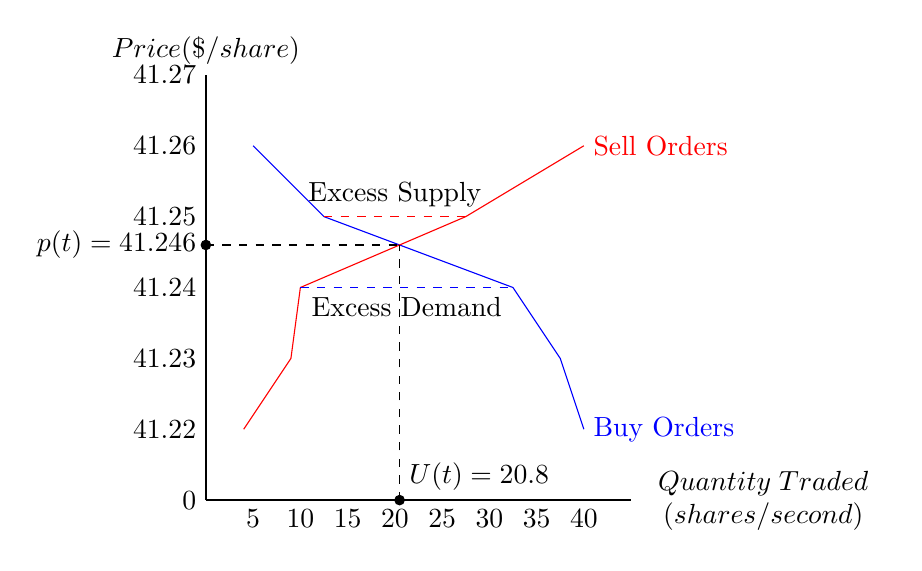
\begin{tikzpicture}[scale=0.6]
            \draw[thick,-] (0,0) -- (0,9) node[above]{$Price (\$/share)$};
            \draw[thick,-] (0,0)--(9,0) node[right]{\begin{tabular}{c}
                 $Quantity \; Traded$ \\
                 $(shares/second)$
            \end{tabular}};
            \node[left] at (0,1.5) {$41.22$};
            \node[left] at (0,3.0) {$41.23$};
            \node[left] at (0,4.5) {$41.24$};
            \node[left] at (0,6.0) {$41.25$};
            \node[left] at (0,7.5) {$41.26$};
            \node[left] at (0,9.0) {$41.27$};
            \node[below] at (1,0) {$5$};
            \node[below] at (2,0) {$10$};
            \node[below] at (3,0) {$15$};
            \node[below] at (4,0) {$20$};
            \node[below] at (5,0) {$25$};
            \node[below] at (6,0) {$30$};
            \node[below] at (7,0) {$35$};
            \node[below] at (8,0) {$40$};
            \node[left] at (0,0) {$0$};
            \draw[blue,solid] (1,7.5) -- (2.5,6.0) -- (6.5,4.5) -- (7.5,3) -- (8,1.5) node[right]{Buy Orders} ;
            \draw[red,solid] (0.8,1.5) -- (1.8,3) -- (2,4.5) -- (5.5,6) -- (8,7.5) node[right]{Sell Orders};
            \draw[red,dashed] (2.5,6.0) -- (5.5,6.0);
            \draw[blue,dashed] (2,4.5) -- (6.5,4.5);
            \node[black,above] at (4,6.0) {Excess Supply};
            \node[black,below] at (4.25,4.5) {Excess Demand};
            \draw[dashed] (4.1,0) -- (4.1,5.4);
            \draw[dashed] (0,5.4) -- (4.1,5.4);
            \node[above right] at (4.1,0) {$U(t)=20.8$};
            \draw[fill] (4.1,0) circle [radius=.1];
            \node[left] at (0,5.4) {$p(t)=41.246$};
            \draw[fill] (0,5.4) circle [radius=.1];
        \end{tikzpicture} \\
\raggedright \footnotesize Note: Excess supply = 28 - 12 = 16 shares at \$41.25 and excess demand = 34 - 10 = 24 shares at the next lower tick, \$41.24, so the clearing price is $\frac{41.24 ^* 16 \ + \ 41.25 ^* 24}{16 \ + \ 24}$ = \$41.246.
        \label{fig:snd}
    \end{figure}

The flow format enables traders to finely tailor their market engagement. Their chosen CSLOs reflect not only their target prices but also their urgency of trading. It is not hard to see that the impact a CSLO has on clearing price is reduced when a trader reduces her $U_{\max}$ or expands the width $P_U- P_L$ of her acceptable price range.  

\bigskip
\noindent
\textbf{FLOW User Interface.} 
The software and interface for the Flow market is analogous to that of the CDA market. 
Figure \ref{fig:exp_interfaces} panel (b) shows one trader's FLOW trading screen.  The trader sets and submits buy and sell orders in the top-middle box (titled ``Your Input''). The horizontal axis denotes \textit{rate} in shares per second, and the vertical axis denotes prices in ECUs per share. The trader sets a \textit{buy} order by moving the blue dot along the vertical axis to set the high price and dragging the blue square anywhere inside the grid to set the low price and the maximum rate. Then, she enters the total number of shares she wants to buy in the box next to the ``Send Buy" blue button and submits it by clicking that button. The blue-line segments graphically describe her buy order. %, as shown in Figure \ref{fig:exp_interfaces} panel (b). 
Likewise, she sets a \textit{sell} order by moving the red dot along the vertical axis to set the low price and dragging the red square anywhere inside the grid to set the high price and the maximum rate. Then, she enters the total number of shares she wants to sell in the box next to the ``Send Sell" red button and submits it by clicking that button. She can submit a new order at any time by canceling her active orders on the same side of the market and then creating a new order. 

The trader sees the market supply (the blue piecewise linear curve) and demand (red) in the top-right Market box. Their intersection determines the clearing price $p(t)$ and the aggregate clearing rate $q(t)$. The green horizontal line at height $p(t)$ in the Market diagram extends into the \textit{Your Input} box and indicates the current market price. The x-coordinate of the intersection of this line and the trader's order indicates the trader's current trading speed. The column of tables on the left side of the interface and the bottom boxes (projected profits, inventory, and cash) are analogous to those in the CDA user interface.  


% \newpage
\begin{figure}
    \centering
    \caption{Experiment Interfaces}
    \begin{subfigure}[b]{\linewidth}
        \centering
        
\includegraphics[width=0.9\linewidth]{figures/cda_ui.png}
        \caption{CDA Format}
        \label{fig:cda_ui}
    \end{subfigure}
    
    \begin{subfigure}[b]{\linewidth}
        \centering
        
\includegraphics[width=0.9\linewidth]{figures/flow_ui.png}
        \caption{FLOW Format}
        \label{fig:flow_ui}
    \end{subfigure}
    \label{fig:exp_interfaces}
\end{figure}
% \newpage

\subsection{Implementation}\label{sect:design}

We implemented a between-group design where each session consists of 20 trading periods, each lasting two minutes. Each market consists of eight traders.  We have 80 participants, 40 trading periods in each market format. Thus there are 5 sessions (or ``groups'') in the CDA format and a perfectly parallel set of 5 sessions in the Flow format. 
That is, each CDA session has a identical twin Flow session with the same pattern of contract assignments, blocks, etc. as detailed below. 

At the start of each market of eight traders, four receive a single buy contract and four receive a sell contract. %as each period starts. 
As mentioned above, %buy and sell contracts are analogous to induced values and costs in standard market experiments. In particular, 
a buy (sell) contract is a commitment from the experimenter to buy (sell) up to $Q_{\textit{contract}}$ units at price $p_{\textit{contract}}$ at the specified expiration time, here at the end of the trading period. % of the contract (all expiration times were set near the end of the trading period). 

We divided the 20 trading periods into five blocks of four consecutive periods each. The four periods have the same contract configuration, i.e., the induced demand and supply curves repeat and so do the quantity and price of equilibrium. The contract configuration changes when the next block begins. We use three different configurations of contracts in the five blocks. The first three blocks have different configurations, and Block four repeats the configuration of Block two, and Block five repeats that of Block one.
Figure \ref{fig:3contract_configs_new} depicts those three contract configurations. %used in our experiment.  
The blue staircases represent the buy contracts, sorted to form the induced demand curve, and the red supply curve similarly represents the sell contracts. 
Each contract assigned to an individual trader is a step (a flat line segment) on either demand or supply curve. 
Within each block, each trader receives the same contract each period. Across blocks, buyers and sellers receive different contracts but keep the same role. % but we assign a new set of contacts as shown in Figure \ref{fig:3contract_configs_new}. 

%%%%% CONTRACT FIGURES %%%%%%%%%

\begin{figure}
    \centering
    % \caption{Contract Configurations}
    \begin{subfigure}[c]{0.33\linewidth}
        \centering
            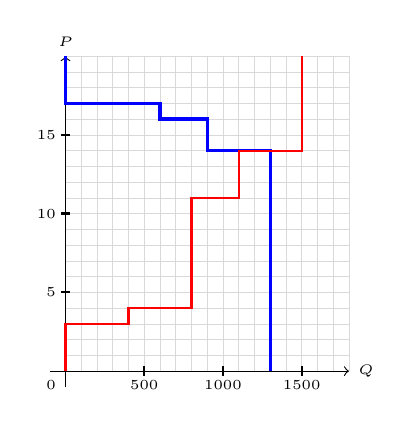
\begin{tikzpicture}[scale=.2]
                % create grid
                \draw[help lines, gray!30] (0,0) grid (18,20);
                
                % Draw axes
                \draw[->] (-1,0) -- (18,0) node[font=\tiny,right] {$Q$};
                \draw[->] (0,-1) -- (0,20) node[font=\tiny,above] {$P$};
              
                % Draw step functions
                \draw[blue, very thick] (0,20) -- (0,17) -- (6,17) -- (6,16) -- (9,16) -- (9,14) - - (13,14) -- (13,0) ;
                \draw[red, thick] (0,0) -- (0,3) -- (4,3) -- (4,4) -- (8,4) -- (8,11) --  (11,11) -- (11,14) -- (15,14) -- (15,20);
                
                % % Add labels
                \node[font=\tiny,below left] at (0,0) {$0$};
                \foreach \x in {5,10,15} {
                  \node[font=\tiny,below] at (\x,0) {$\x00$};
                }
                \foreach \y in {5,10,15} {
                  \node[font=\tiny,left] at (0,\y) {$\y$};
                }
                
                % % Add thicker ticks (Q)
                \draw[black, thick] (5,-0.3) -- (5,0.3);
                \draw[black, thick] (10,-0.3) -- (10,0.3);
                \draw[black, thick] (15,-0.3) -- (15,0.3);

                % % Add thicker ticks (P)
                \draw[black, thick] (-0.3,5) -- (0.3,5);
                \draw[black, thick] (-0.3,10) -- (0.3,10);
                \draw[black, thick] (-0.3,15) -- (0.3,15);
            \end{tikzpicture}
        \subcaption{\tiny Block 1 (T1-T4) \\ and Block 5 (T17-T20)}
    \end{subfigure}%
    \begin{subfigure}[c]{0.33\linewidth}
        \centering
        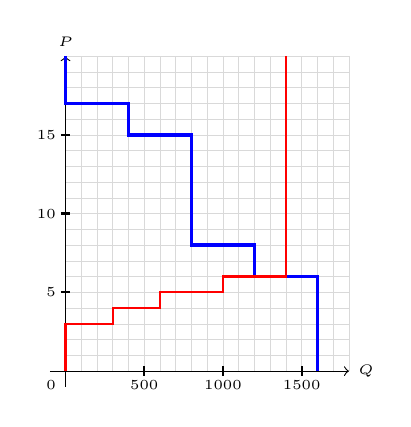
\begin{tikzpicture}[scale=.2]
            % create grid
            \draw[help lines, gray!30] (0,0) grid (18,20);
            
            % Draw axes
            \draw[->] (-1,0) -- (18,0) node[font=\tiny,right] {$Q$};
            \draw[->] (0,-1) -- (0,20) node[font=\tiny,above] {$P$};
          
            % Draw step functions
            \draw[blue, very thick] (0,20) -- (0,17) -- (4,17) -- (4,15) -- (8,15) -- (8,8) -- (12,8) -- (12,6) -- (16,6) -- (16,0);
            \draw[red, thick] (0,0) -- (0,3) -- (3,3) -- (3,4) -- (6,4) -- (6,5) -- (10,5) -- (10,6) -- (14,6) -- (14,20);
            
            % % Add labels
            \node[font=\tiny,below left] at (0,0) {$0$};
            \foreach \x in {5,10,15} {
              \node[font=\tiny,below] at (\x,0) {$\x00$};
            }
            \foreach \y in {5,10,15} {
              \node[font=\tiny,left] at (0,\y) {$\y$};
            }

            % % Add thicker ticks (Q)
            \draw[black, thick] (5,-0.3) -- (5,0.3);
            \draw[black, thick] (10,-0.3) -- (10,0.3);
            \draw[black, thick] (15,-0.3) -- (15,0.3);

            % % Add thicker ticks (P)
            \draw[black, thick] (-0.3,5) -- (0.3,5);
            \draw[black, thick] (-0.3,10) -- (0.3,10);
            \draw[black, thick] (-0.3,15) -- (0.3,15);
        \end{tikzpicture}
        \subcaption{\tiny Block 2 (T5-T8) \\ and Block 4 (T13-T16)}
    \end{subfigure}%
    \begin{subfigure}[c]{0.33\linewidth}
        \centering
        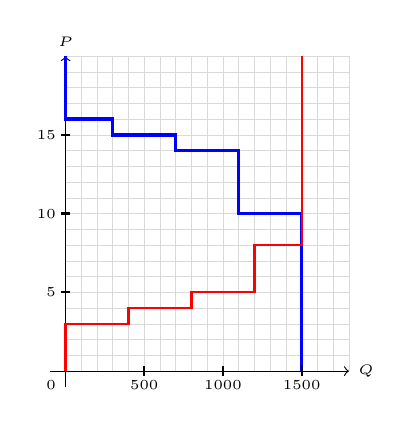
\begin{tikzpicture}[scale=.2]
            % create grid
            \draw[help lines, gray!30] (0,0) grid (18,20);
            
            % Draw axes
            \draw[->] (-1,0) -- (18,0) node[font=\tiny,right] {$Q$};
            \draw[->] (0,-1) -- (0,20) node[font=\tiny,above] {$P$};
          
            % Draw step functions
            \draw[blue, very thick] (0,20) -- (0,16) -- (3,16) -- (3,15) -- (7,15) -- (7,14) -- (11,14) -- (11,10) -- (15,10) -- (15,0);
            \draw[red, thick] (0,0) -- (0,3) -- (4,3) -- (4,4) -- (8,4) -- (8,5) -- (12,5) -- (12,8) -- (15,8) -- (15,20);
            
            % % Add labels
            \node[font=\tiny,below left] at (0,0) {$0$};
            \foreach \x in {5,10,15} {
              \node[font=\tiny,below] at (\x,0) {$\x00$};
            }
            \foreach \y in {5,10,15} {
              \node[font=\tiny,left] at (0,\y) {$\y$};
            }

            % % Add thicker ticks (Q)
            \draw[black, thick] (5,-0.3) -- (5,0.3);
            \draw[black, thick] (10,-0.3) -- (10,0.3);
            \draw[black, thick] (15,-0.3) -- (15,0.3);

            % % Add thicker ticks (P)
            \draw[black, thick] (-0.3,5) -- (0.3,5);
            \draw[black, thick] (-0.3,10) -- (0.3,10);
            \draw[black, thick] (-0.3,15) -- (0.3,15);
        \end{tikzpicture}
        \subcaption{\tiny Block 3 (T9 - T12)}
    \end{subfigure}
    \caption{\textbf{Contract configurations across trading blocks.}  \footnotesize
Vertical axis is price (ECU per share) and horizontal axis is quantity (shares). Each panel plots the step‐function demand schedule (thick blue) and supply schedule (red).  
The intersection of the two schedules determines the competitive‐equilibrium price–quantity pair for that block.  
Panel (a) applies to Blocks 1 (T1–T4) and 5 (T17–T20) of experiment; panel (b) to Blocks 2 (T5–T8) and 4 (T13–T16); panel (c) to Block 3 (T9–T12). }
% \label{fig:contract-configs}
    \label{fig:3contract_configs_new}
\end{figure}

% Yilin please add captions explaining the blocks and the equilibrium values. 

Experiment instructions were provided on the computer screen and paper; see Appendices \ref{app_instruction_cda} and \ref{app_instruction_flow} for a copy. % Instructions were discussed and piloted (with students and colleagues) to balance clarity and reasonable length.} 
% \footnote{To ensure clarity and understanding of the experiment's rules and objectives, we provided participants with detailed instructions on-screen and paper, supplemented by a video summary. The experiment also included trial periods for participants to familiarize themselves with the interface and market rules. Final payments were based on accumulated wealth, incorporating a fixed participation fee.}
After 15 minutes of reading instructions, a video summary was played with animations and annotations to clarify any confusion that subjects might have.
Subjects next participated in two 120-second trial periods to familiarize them with the interface and market rules, and were then invited to ask any questions.
Subjects were not allowed to communicate with each other before or during the experiment, nor did they learn the identity or characteristics of other participants.

In between trading periods, each subject viewed a summary screen displaying a profit history of each the previous trading period.
% KLV Should we add a screen in the appendix?
Each participant started each trading period with a zero endowment. Final payments were based on the final accumulated wealth of all twenty trading periods, using an exchange rate of 1000 ECUs = \$1, plus a \$7 participant fee. This information was provided to subjects in the written instructions.
Although ending a trading period with negative profits is possible (i.e., having negative ECUs in the period), this happened in less than 5\% of cases
%4.62\% of the cases (4.88\% in CDA and 4.37\% in FLOW)
and subjects never left the laboratory with less than \$7. Payments were implemented following standard confidentiality procedures. 
% KLV how about total negative wealth? Did that happen?
The experiment software was built on the oTree platform (\cite{otree}). Sessions were conducted at the LEEPS Laboratory of the University of California, Santa Cruz. Subjects were recruited via LEEPS' ORSEE instance (\hyperlink{https://econlab.ucsc.edu/public/}{econlab.ucsc.edu}; \cite{subject}).


% \subsection{Hypotheses}
% list the criteria we will use for market quality  --- 
% allocative efficiency, price efficiency, price volatility, profit level and dispersion, ... ---
% and for each criterion offer a hypothesis on which format will be better.

% describe in words how we defined?
%%%%%%%%%%%%%%%%%%%%%%%%%%%%%%%%%%%%%%%%%%%%%%%%%%%%%%%%%%%%%%%%%%%%%%%%%%%%%%%%%%%%%%%%%%%%%%%%%%%%%%%%%%%%%%%%%%%
\subsection{Performance Metrics and Hypotheses}\label{sect:metricHyps}
\label{sec:hypotheses}

To compare the two market formats, we will analyze \textbf{trading behavior} in terms of 
the \textit{number of submitted orders} per trading period, 
the \textit{size of submitted orders}  in shares per order,
the \textit{prices} of the limit orders in CDA or the continuous scaled limit orders in Flow, and
the \textit{maximum trading rate} specified in a CSLO.
We will also analyze \textbf{market performance} in terms of the following metrics.
\textit{Absolute Price Change} is defined for each period as the average absolute price difference between adjacent time grid points, $|P_t - P_{t-1}|$. A larger value indicates more erratic prices. 
Our convention on
the (5 second) time grid is described below. %lower price volatility. %\footnote{We define trading intervals at the beginning of the Results section.}
\textit{Price volatility} is defined for each period as the variability of proportional price changes and calculated as the standard deviation of $(\ln P_t - \ln P_{t-1})$ across time grid intervals.  %periods and groups. This is another metric of price volatility. 
\textit{Trade Volume} is defined  as the total quantity of shares traded in a period. It is an aggregate indicator of market activity, and can be compared to the minimum trading volume required to achieve a competitive equilibrium allocation. An alternative volume metric is the fraction of contract quantity that is filled; this alternative metric eliminates volume due to ``churn,'' e.g.,  traders reselling part of their purchases.
\textit{Informational [in]efficiency} is  defined each period as the mean distance between transaction price and the  competitive equilibrium price, \( |P_t - P_{\text{CE}}| \). It reflects the market's ability to incorporate into price all private information regarding supply and demand (here, unexpired contracts); 
smaller deviations from  competitive equilibrium price indicate higher informational efficiency.
Finally, \textit{Allocative efficiency} is measured as \( \Pi/\Pi_{\text{CE}}\), i.e.,
 realized surplus (the sum of traders' actual profits) as a fraction of potential surplus (the sum of trader profits earned in competitive equilibrium). 
This metric assesses how efficient the market is in extracting potential gains from trade.       


%%%%%%%%%%%%%%%%%%%%%%%%%%%%%%%%%%%%%%
% \vspace{0.5cm}
% \noindent \textit{Hypotheses} \\

These metrics allow us to formulate the following testable hypotheses. 

%\vspace{0.3cm}
\noindent \textbf{Hypothesis 1: Order shredding.} \textit{Traders will submit a larger number of smaller quantity orders in CDA format than in Flow format.} 
%\vspace{0.3cm}

\noindent As discussed earlier, to reduce price impact in the CDA, traders have to shred their orders manually, i.e., to break them into small fragments submitted sequentially. By contrast, the Flow format automatically facilitates very fine order shredding since, in each short time interval, only a very limited quantity can be transacted. 
The Flow format can closely reproduce CDA trading and pricing dynamics if traders minimize the separation between $P_L$ and $P_H$ and submit the highest allowed trading rate, ($U_{\text{max}}=30$ shares per second). 
If traders instead modulate their urgency to trade --- by setting substantial distances between $P_L$ and $P_H$ prices and/or choosing maximum execution rates, $U_{\text{max}}$, well below the highest rate allowed by the interface --- then they automatically will greatly reduce price impact even when they submit large orders. Thus, if traders care about price impact,
in the Flow format we should observe fewer but larger orders than in the CDA. 

%\vspace{0.3cm}
\noindent \textbf{Hypothesis 2: Volatility.} \textit{Price volatility will be lower with the Flow format than with the CDA.}
%\vspace{0.3cm}

\noindent In the CDA, each transaction is executed at a price determined by a unique matching of  limit orders of a buyer and a seller. This can lead to a wide dispersion of transaction prices within a short time frame. In contrast, the Flow Market operates under a uniform pricing rule — from moment to moment, every trade for every active trader is executed at the same price, until an active order is fully filled or a new order arrives. This uniformity may attenuate transaction price fluctuations, yielding a more stable price path. Hence, we hypothesize that the Flow format brings lower price volatility than the CDA. 

\vspace{0.3cm}
\noindent \textbf{Hypothesis 3: Volume.} \textit{The CDA and Flow formats will exhibit similar levels of trade volume. }
%(b) Both will move within each trading block towards the minimum volume that sustains competitive equilibrium.} 
%\vspace{0.3cm}

\noindent There is no obvious reason why the overall trade volume should be larger in one format than the other, so H3 is the natural null hypothesis. We shall also examine whether trade volume in later periods approaches the competitive equilibrium volume. 

\vspace{0.3cm}
\noindent \textbf{Hypothesis 4: Efficiency.} \textit{The CDA and Flow formats will exhibit similar levels of (a) informational and (b) allocative efficiency.} 
%\vspace{0.3cm}

\noindent Again, there is no compelling \textit{a priori} reason to expect one format to be more efficient than the other, either in informational efficiency (prices close to competitive equilibrium) or in allocative efficiency (near exhaustion of gains from trade),\footnote{Note this is not necessarily true in environments such as \cite{Budish2015, Aldrich2019} where equilibrium in CDA implies socially wasteful investment in technology.}
so H4 is the natural null hypothesis.
On the other hand, proponents of either format would be happy to see this hypothesis rejected in their preferred direction.

%%%%%%%%%%%%%%%%%%%%%%%%%%%%%%%%%%%%%%%%%%%%%%%%%%%%%%%%%%%%
%%%%%%%%%%%%%%%%%%%%%%%%%%%%%%%%%%%%%%%%%%%%%%%%%%%%%%%%%%%%

\section{Results} \label{results}


We start with descriptive statistics of trader behavior and market performance. Section \ref{sect:RegResults} then will present regression results, including formal tests of Hypotheses H1 - H4.

\subsection{Descriptive statistics}

%%% Traders' Behavior 
%\vspace{0.5cm}
\noindent \textbf{Trader Behavior.} 
Table \ref{tab:summary_stat_trader} suggests that trader behavior in the Continuous Double Auction (CDA) 
diverges sharply from that in the Flow Market format. 
An average of 32 orders per period were observed in the CDA market, while the Flow Market averaged only 24 orders. % That is, traders in the CDA market exhibited a higher frequency of order placements. We then look into the average quantity submitted per order. 
On the other hand, the Flow Market averages a substantially larger order size at 182 shares per order, while the CDA averages only 113 shares. This divergence persists in both early (T1-10) and late (T11-20) sessions and for Buyers as well as Sellers. Although not a formal test of H1, the descriptive statistics suggest that indeed the Flow market's automatic shredding helps traders reduce price impact without having to chop up their orders manually.  

The rest of the Table shows both similarities and divergences in pricing behavior. 
Bid prices in the CDA market average 6.9 ECU per share, while Flow Market bid prices stretch from an average minimum of 4.22 to an average maximum of 9.71. Thus the CDA average submitted bid is precisely in the middle of Flows' min and max prices. The pattern, however, is quite different for sellers. Their average submitted ask price in the CDA is 10.7 ECU, while in the Flow Market, average min ask prices is only a bit lower at 9.21 and the average ask is much higher at 15.46. 
We will see later that this order price asymmetry 
leads to profit asymmetries between buyers and sellers. 




% \begin{table}[!htbp]
\begin{table}
    \centering
    \caption{Summary Statistics: Traders' Behavior}
    \renewcommand{\arraystretch}{1}
    \resizebox{1\textwidth}{!}{
    \begin{threeparttable}
    \begin{tabular}{lcccccc}
    \toprule
    ~                               & \multicolumn{2}{c}{T1 - T20} & \multicolumn{2}{c}{T1 - T10}  & \multicolumn{2}{c}{T11 - T20} \\
                                    & CDA       & FLOW      & CDA       & FLOW      & CDA       & FLOW      \\
    \midrule ↩
    % \multicolumn{7}{l}{\textbf{(a) Trader Behavior}} \\
    % \hline \\[-1.8ex]
     Number of Orders                       & 32       & 24            & 31       & 25            & 32        & 23            \\
     \hspace{3mm}Seller             & 17       & 12            & 17       & 13            & 17        & 11            \\
     \hspace{3mm}Buyer              & 15       & 12            & 15       & 12            & 15        & 12            \\
     % Order Size                     & 42       & 72            & 44       & 63            & 40        & 80            \\
     \\
     Quant. per Order                 & 113      & 182           & 115      & 180           & 111       & 185           \\
     \hspace{3mm}Seller             & 115      & 185           & 118      & 184           & 111       & 185           \\
     \hspace{3mm}Buyer              & 114      & 188           & 116      & 184           & 113       & 191           \\
     \\
     Order Price                    & 8.93     & [6.78, 12.64] & 9.18     & [7.15, 13.01] & 8.68      & [6.41, 12.28] \\
     \hspace{3mm}Seller             & 10.7     & [9.21, 15.46] & 11.13    & [9.76, 16.04] & 10.27     & [8.66, 14.88] \\
     \hspace{3mm}Buyer              & 6.9      & [4.22, 9.71]  & 7.01     & [4.26, 9.71]  & 6.79      & [4.19, 9.71]  \\

    \\
     Order Max Rate                 &           & 19.62         &           & 17.78         &           & 21.46         \\
     \hspace{3mm}Seller             &           & 19.67         &           & 18.06         &           & 21.29         \\
     \hspace{3mm}Buyer              &           & 20.15         &           & 17.93         &           & 22.37         \\
    \bottomrule
    \end{tabular}
    \begin{tablenotes}
    \item \small \textit{Notes:} 
%T1-T20 indicates all periods, 
T1-10 indicates the first 10 periods in each session and T11-20 indicates the last 10 periods.
All reported statistics are averages across time intervals, periods and groups.
The Quantity per Order reflects the average quantity of shares submitted per order.
    Order Price shows the mean order price for CDA. The brackets indicate the average minimum and maximum price submitted in Flow orders. Order Max Rate is the maximum trading speed submitted in Flow orders. 
    \end{tablenotes}
    \end{threeparttable}
    }
    \label{tab:summary_stat_trader}
\end{table}

It is also worth noting that the wide difference between average minimum and maximum order price --- for both buyers and sellers --- suggests that traders indeed seize the richer possibilities the Flow format  provides to modulate immediacy.  
That impression is corroborated by the fact that the average maximum rates in Flow bid and ask orders (20.15 and 19.67 respectively)
are well short of the maximum allowed (30.0).
%The fact that, in all cases for Flow markets, there is a wide separation between the average minimum and maximum price  suggests that traders generally understood and used the more expressive options that the Flow market format provides. 
On the other hand, the chosen max rates do increase, from 17.78 on average in the initial half to 21.46 in the latter half of a session. This is the only order component in either Flow or CDA that changes much from the first to the second half of the session. 

%%%%%%
% Market Performance
\vspace{0.5cm}
\noindent \textbf{Market Performance.} 
Table \ref{tab:summary_stat} presents summary statistics of market performance. To create comparability between the Continuous Double Auction (CDA) and the Flow Market (FLOW), we split each trading period into twenty-four 5-second intervals, and within each interval, we compute traded quantity-weighted average transaction prices. 
Panel (a) of Table \ref{tab:summary_stat} %details the average prices and their volatility. The Flow market exhibits 
shows higher average transaction prices in Flow markets, with an overall mean of 9.37 ECUs, compared to the CDA’s average of 8.62, both short of the average competitive equilibrium (CE) price of 9.8. %\footnote{Below, we discuss the associated metric of information (price) efficiency.}
%Interestingly, the average size and variability of price changes are consistently lower under Flow than under CDA, 



% \begin{table}[!htbp]
\begin{table}
    \centering
    \caption{Summary Statistics: Market Performance}
    \renewcommand{\arraystretch}{1.1}
    % \resizebox{.75\textwidth}{!}{
    \begin{threeparttable}
    \begin{tabular}{lcccccc}
    
    \toprule
    
    ~                               & \multicolumn{2}{c}{T1 - T20} & \multicolumn{2}{c}{T1 - T10}  & \multicolumn{2}{c}{T11 - T20} \\
                                    & CDA       & FLOW      & CDA       & FLOW      & CDA       & FLOW      \\
    \midrule 
     \\[-1.8ex] 
     \multicolumn{7}{l}{\textit{\textbf{(a)} Price Statistics} (Avg. Equil Price = $9.8$ ECUs)} \\
    % \hline 
     \\[-1.8ex]    
     Clearing Prices ($P_t$, ECUs)              & 8.62      & 9.37      & 9.04      & 9.57      & 8.21      & 9.18      \\
     \hspace{3mm}(Std. Dev.)                    & (2.77)    & (2.54)    & (2.95)    & (2.75)    & (2.51)    & (2.29)    \\
     $ \lvert  P_{t}-P_{t - 1} \rvert $         & 0.57      & 0.39      & 0.58      & 0.39      & 0.55      & 0.4       \\
     Std. Dev. of $(\ln P_{t} - \ln P_{t - 1})$ & 0.14      & 0.07      & 0.15      & 0.07      & 0.13      & 0.07      \\     
     \\ [-1.8ex]
     \multicolumn{7}{l}{\textit{\textbf{(b)} Volume, Transaction Intensity}} \\
     \\ [-1.8ex]
     Trade Volume (shares)                     & 1138      & 959       & 1097      & 872       & 1179      & 1046      \\
     Trade Vol. / $Q_{\text{CE}}$. (\%)        & 93.6      & 78.8      & 90.3      & 71.1      & 96.9      & 86.4      \\
     Filled Contract / $Q_{\text{CE}}$ (\%)     & 85.2      & 77.1      & 81.0      & 69.8      & 89.3      & 84.5      \\
     Num. of Transactions                             & 14        &           & 13        &           & 15        &           \\
     Mean Transaction Size                      & 78        &           & 82        &           & 74        &           \\
     \hspace{3mm}(Std. Dev.)             & (61)      &           & (61)      &           & (60)      &           \\
     Clearing Rate ($q/sec$)                 &           & 9.37      &           & 9.54      &           & 9.2       \\
     \hspace{3mm}(Std. Dev.)             &           & (2.6)     &           & (2.8)     &           & (2.4)     \\
     \\ [-1.8ex]
     \multicolumn{7}{l}{\textit{\textbf{(c)} Efficiency and Buyer-Seller Inequality}} \\
     \\ [-1.8ex]
     Info. Effic.: $\lvert P_t - P_{\text{CE}} \rvert $        & 2.16      & 2.08      & 2.19      & 2.32      & 2.14      & 1.84      \\     
     Alloc. Effic.: $\Pi$ / $\Pi_{\text{CE}}$ ($\times 100$)          & 84.3      & 81.81     & 79.76     & 77.31     & 88.85     & 86.31     \\
     
     ${\Pi^{\text{buy}}}/{\Pi^{\text{buy}}_{\text{CE}}} - {\Pi^{\text{sell}}}/{\Pi^{\text{sell}}_{\text{CE}}}$ 
     ($\times 100$) & 53.7      & 11.18     & 27.38     & -5.16     & 80.03     & 27.51     \\
     \\[-1.8ex] 
    \bottomrule 
    \end{tabular}
    \begin{tablenotes}[para,flushleft]
      \footnotesize
\textit{Note:} All price sequences are quantity-weighted within 5-second intervals, then averaged over all periods and groups. \( |P_{t} - P_{t-1}| \) represents average absolute price changes between intervals. Standard Deviation of \( \ln P_{t} - \ln P_{t-1} \) is a volatility measure for proportional price changes between the intervals. Trade Volume / $Q_{CE}$ (as \%) indicates average total quantity transacted per period relative to the minimum required to reach competitive equilibrium (CE). Filled Contract / $Q_{CE}$ (as \%) is the total quantity bought (or sold) when all contracts expired and were executed. 
Num. of Transactions and Mean Transaction Size are CDA averages rounded to nearest integer. 
The clearing rate reflects the intensity of Flow trading. 
Informational efficiency, \( |P_{t} - P_{CE}| \), and allocation efficiency, \( \Pi/\Pi_{CE} \times 100 \)
are averaged across trading periods.
The last line is profit asymmetry, the difference \( (\Pi^{buy}/\Pi^{buy}_{CE} - \Pi^{sell}/\Pi^{sell}_{CE}) \times 100 \) in normalized (relative to CE) profits between buyers and sellers. 
    \end{tablenotes}
    \end{threeparttable}
   % }
    \label{tab:summary_stat}
\end{table}

The Table strongly suggests greater price stability with the Flow format. 
Its overall average absolute price change (\(|P_t - P_{t-1}|\)) is 0.39 ECUs versus 0.57 in the CDA.  %The same pattern applies when comparing the sessions' first half (T1 - T10) and the second half (T11 - T20).
The contrast in average price volatility (standard deviation of log of price changes) is even sharper:
just 0.07 in Flow versus 0.14 in CDA.
Both contrasts are consistent across the two halves of the trading period. %These figures show consistently lower volatility in price changes in the Flow market, pointing at traders in Flow experiencing a more predictable price evolution. 

Figure \ref{fig:price} displays the session-level price data in each 5 second time interval.  %YL: i need to double check, this should be raw prices if i remembered correctly
Light color dots and lines represent transaction prices in individual sessions and the darker green lines or dots are averages over sessions. The pink horizontal lines represent the underlying equilibrium prices. %Panel (a) displays the data for CDA, and Panel (b) for the Flow market. 
We note considerable variation across sessions, with the average price highlighting an overall under-reaction to changes in the competitive equilibrium price, particularly within CDA markets
(Panel a). The last block suggests again that Flow markets (shown in Panel b of Figure \ref{fig:price}) eventually track CE price slightly better than do CDA markets, although neither performance is impressive.

The volume and transaction intensity measures shown in Panel (b) of Table~\ref{tab:summary_stat}
may also be of interest.
In the CDA format, trade volume as a fraction of competitive equilibrium (CE) quantity increases from 90.3\% in the first ten periods to 96.9\% in the latter ten (T11-T20), an increase of 6.6 percentage points. Volume in Flow increases more sharply, by 15.3 percentage points, but starts much lower, at 71.1\%. % to 86.4\%, for a  percentage point increase for Flow versus 6.6 for CDA.
This suggests a more substantial adaptation by traders in the Flow format as they gain experience. 
One might think that volume in both formats is converging towards CE levels, and this impression seems consistent with  Figures \ref{fig:surplus_volume}(a) and (b).
%, where the traded volume in CDA and Flow are depicted across periods. 
Very similar patterns are seen in 
the alternative measure, filled contracts as a percentage of competitive equilibrium quantity (\(Q_{CE}\)), eliminates churn (retrading) but still exhibits very similar patterns. 
%Again there is a greater increase for Flow from a smaller value in T1-T10.
%In the CDA, there is an increase in this metric, which climbs from 81.0\% in the initial half of the sessions to 89.3\% in the latter half. In the Flow market, this metric starts at a lower value of 69.8\% and then climbs rapidly to 84.5\%.

The number of CDA transactions per period increases only slightly from 13 in the first ten periods of a session to 15 in the last ten. On the other hand, the Mean Transaction Size in CDA  decreases from an average size of 82 shares in T1-T10 to 74 shares in T11-T20 (albeit with considerable variability; the coefficient of variation ($\frac{Std. Dev}{Mean}$) is around 0.75.) 
These trends may suggest increasing strategic fragmentation of orders
(shredding) over time in the CDA.
A parallel trend in the Flow markets is suggested by its average clearing rate far below the upper limit of 30 shares per second, with a slight decrease from 9.5 in the first half to 9.2 in the second half of a session. 

Panel (c) in the same table reveals each market format's efficiency. Recall that informational efficiency, $\lvert P_t - P_{\text{CE}} \rvert $, captures the market's capacity to track  equilibrium price, while  allocation efficiency,  $\Pi$ / $\Pi_{\text{CE}}$ ($\times 100$), is the percentage of potential CE surplus that is realized in each trading period. The Table indicates that the two formats perform similarly in the second half of the sessions, after participants have learned and gained experience. %In information efficiency, while CDA exhibits an average absolute deviation from the $P_{\text{CE}}$ of $2.14$, the Flow format exhibits an average deviation of $1.84$ (although in the first half, Flow performs slightly worse than CDA). In allocative efficiency, while CDA exhibits an average percentage of realized surplus of $88.9 \%$, the Flow format exhibits an average deviation of $86.3 \%$ (in the first half of the session, these measures were 84.3\% and 81.8\%, respectively). 
Overall, it seems that the CDA displays slightly higher allocation efficiency, while Flow exhibits slightly higher information efficiency. The levels are not as high as one typically observes in classic laboratory environments with one way trade of only a few indivisible units, but are comparable to other experiments [cite?] where traders can both buy and sell highly divisible asset units.

Finally, Panel (c) of Table \ref{tab:summary_stat} and Figure \ref{fig:norm_profits}  document the patterns of profit distributions across market formats. We find that profits are more evenly distributed in Flow than in CDA, where buyers' normalized profits greatly exceed sellers' profits. That is, even though the realized surplus is on average slightly higher in CDA than in Flow, the difference between buyers and sellers is much smaller in Flow. 
Figure~\ref{fig:norm_profits}) shows that buyers tend to earn more than competitive equilibrium profits in CDA, with around 40\% earning at least one and a half times the CE profits, especially in the second half. 



% %%%%%%%% 

% Table \ref{tab:summary_stat} reports summary statistics for the experiment. 
% To maintain better comparability across formats, we break each trading period into 24 five-second intervals.
% Since transaction sizes vary quite widely, in each interval we compute the transaction quantity-weighted average price. 

% Panel (a) of the Table reports statistics obtained from those 24 observations per period, beginning with their overall average and standard deviation.
% Overall (and also in both the first 10 and the last 10 periods) prices are slightly higher in Flow than in CDA trading periods, and standard deviations are slightly lower.
% The next two lines of the Table show that on average price changes are roughly one and a half times larger in CDA as in FLOW and that price volatility is about twice as large. 

% Panel (b) of \ref{tab:summary_stat} summarizes order and transaction quantities. 
% Traded volume as a fraction of the CE quantity is notably larger in the CDA in periods 1-10, but the increase in periods 11-20 is larger in FLOW.
% The percentage of filled CE quantity also trends upward, and FLOW eliminates more than half of its shortfall from CDA in the last 10 periods.  
% We consistently see more but smaller orders placed in CDA than in Flow, especially in periods 11-20. 
% Figure \ref{fig:surplus_volume} shows the underlying trends. 
% Again there is considerable heterogeneity across groups, but there is a clear tendency towards the CE surplus (i.e., higher efficiency) and CE volume across blocks, perhaps especially in FLOW sessions. 
% \hl{added metrics of orders?}
% We see that the clearing rate in FLOW is 9.5 shares per second in periods 1-10 but decreases slightly by 0.3 share per second in periods 11-20. 
% The mean transaction size in CDA is 82 shares in periods 1-10 but decreases slightly in periods 11-20 with a slight increase in the average number of transactions.

% Panel (c) of \ref{tab:summary_stat} shows measures of efficiency. 
% Recall that CE prices ranged from 6 to 14, depending on the block. 
% The first line in this panel shows the mean absolute price deviation from CE were rather large but declined slightly in CDA markets, from 2.19 in periods 1-10 to 2.14 in periods 11-20. 
% Price deviations in FLOW markets were larger at 2.32 in periods 1-10 but declined faster to 1.84 in periods 11-20. 
% Figure \ref{fig:price} shows the evolution of prices over time in all sessions (in faint colors) and session averages (dark green).
% There is considerable variation across sessions, but one sees a general tendency to under-respond to shifts in CE price across blocks. 
% Looking at the last block confirms the impression that FLOW markets eventually track CE a bit better than do CDA markets, although neither performance is especially impressive. 
% The last row of the table gives a first glimpse of allocative efficiency.
% In the CDA, average efficiency rises from about 80\% in the first 10 periods to almost 89\% in the last 10. 
% Efficiency also rises by about 9 percentage points in FLOW, but remains 2 or 3 percentage points behind. Figure \ref{fig:norm_profits} compares realized surplus across trader roles and market formats. 
% Even though the realized surplus is always slightly higher in CDA than in FLOW, the difference between buyers and sellers is much smaller in FLOW. Buyers tend to earn more than competitive equilibrium profits in CDA, with around 40\% earning at least one and a half times the CE profits, especially in the second half. 








\begin{figure} 
    \centering
    \begin{subfigure}[b]{\linewidth}
        \centering
        \begin{adjustbox}{trim=0 {.02\height} 0 {.12\height}, clip=true}
            
\includegraphics[width=1\linewidth]{figures/groups_cda_price.png}
        \end{adjustbox}
        \subcaption{\tiny CDA}
    \end{subfigure}
    \begin{subfigure}[b]{\linewidth}
        \centering
        \begin{adjustbox}{trim=0 {.02\height} 0 {.12\height}, clip=true}
            
\includegraphics[width=1\linewidth]{figures/groups_flow_price.png}
        \end{adjustbox}
        \subcaption{\tiny FLOW}
    \end{subfigure} 
    \caption{Clearing Prices. \footnotesize The plot displays observed prices along the whole session, with vertical lines separating each of the 20 paid periods. Lighter color dots and lines represent the prices observed in each session and the darker green lines or dots represent the average prices. The pink lines represent the underlying equilibrium prices. Panel (a) displays the data for CDA and Panel (b) for the Flow market.}    
    \label{fig:price}
\end{figure}

% \vspace{-30pt}
\begin{figure} 
    \centering
    \begin{subfigure}[b]{.5\linewidth}
        \centering
        \begin{adjustbox}{trim=0 {.02\height} 0 {.11\height}, clip=true}
            
\includegraphics[width=\linewidth]{figures/groups_cda_quantity.png}
        \end{adjustbox}
        \subcaption{\tiny CDA Traded Volume}
        \label{fig:cda_volume}
    \end{subfigure}%
    \begin{subfigure}[b]{.5\linewidth}
        \centering
        \begin{adjustbox}{trim=0 {.02\height} 0 {.11\height}, clip=true}
            
\includegraphics[width=\linewidth]{figures/groups_flow_quantity.png}
        \end{adjustbox}
        \subcaption{\tiny FLOW Traded Volume}
        \label{fig:flow_volume}
    \end{subfigure}
    \begin{subfigure}[b]{.5\linewidth}
        \centering
        \begin{adjustbox}{trim=0 {.02\height} 0 {.11\height}, clip=true}
            
\includegraphics[width=1\linewidth]{figures/groups_cda_surplus.png}
        \end{adjustbox}
        \subcaption{\tiny CDA Surplus}
        \label{fig:cda_surplus}
    \end{subfigure}%
    \begin{subfigure}[b]{.5\linewidth}
        \centering
        \begin{adjustbox}{trim=0 {.02\height} 0 {.11\height}, clip=true}
            
\includegraphics[width=1\linewidth]{figures/groups_flow_surplus.png}
        \end{adjustbox}
        \subcaption{\tiny FLOW Surplus}
            \label{fig:flow_surplus}
    \end{subfigure}
    \caption{Traded Volume and Realized Surplus. \footnotesize The plot displays observed volume and surplus along the 20 period of each session. Lighter lines represent the prices observed in each market and the darker green lines represent the average statistics. The pink discontinuous lines represent the underlying equilibrium level. Panel (a) displays the statistics for CDA and Panel (b) for the Flow market.}
    % \begin{subfigure}[b]{.5\linewidth}
    %     \centering
    %     \begin{adjustbox}{trim=0 {.02\height} 0 {.11\height}, clip=true}
    %         
\includegraphics[width=\linewidth]{figures/groups_cda_contract.png}
    %     \end{adjustbox}
    %     \subcaption{\tiny CDA Traded / CE Quantity}
    %     \label{fig:cda_contract}
    % \end{subfigure}%
    % \begin{subfigure}[b]{.5\linewidth}
    %     \centering
    %     \begin{adjustbox}{trim=0 {.02\height} 0 {.11\height}, clip=true}
    %         
\includegraphics[width=\linewidth]{figures/groups_flow_contract.png}
    %     \end{adjustbox}
    %     \subcaption{\tiny FLOW Traded / CE Quantity}
    %     \label{fig:flow_contract}
    % \end{subfigure}
    \label{fig:surplus_volume}
\end{figure}



% \begin{figure}[!htbp] 
%     \centering
%     \caption{Profit Distribution}
%     \begin{subfigure}[b]{.5\linewidth}
%         \centering
%         \begin{adjustbox}{trim=0 0 0 {.11\height}, clip=true}
%             
\includegraphics[width=\linewidth]{figures/gross_profits_cdf.png}
%         \end{adjustbox}
%         \subcaption{\tiny Gross CDF}
%     \end{subfigure}%
%     \begin{subfigure}[b]{.5\linewidth}
%         \centering
%         \begin{adjustbox}{trim=0 0 0 {.11\height}, clip=true}
%             
\includegraphics[width=\linewidth]{figures/excess_profits_cdf.png}
%         \end{adjustbox}
%         \subcaption{\tiny Excess CDF}
%     \end{subfigure}
%     \label{fig:profits}
% \end{figure}

% \begin{figure}[!htbp] 
\begin{figure}
    \centering
    \begin{subfigure}[b]{.5\linewidth}
        \centering
        \begin{adjustbox}{trim=0 0 0 {.11\height}, clip=true}
            
\includegraphics[width=\linewidth]{figures/group_gross_profits_cdf.png}
        \end{adjustbox}
        \subcaption{\tiny T1-T20}
    \end{subfigure}%
    \begin{subfigure}[b]{.5\linewidth}
        \centering
        \begin{adjustbox}{trim=0 0 0 {.11\height}, clip=true}
            
\includegraphics[width=\linewidth]{figures/group_gross_profits_last_cdf.png}
        \end{adjustbox}
        \subcaption{\tiny T11-T20}
    \end{subfigure}
    \caption{Profit Distribution. \footnotesize Panel (a) shows the period-level distribution of profits for the first half of the session and Panel (b) for the second half. We separate the empirical cumulative distributions by market role (seller and buyer) market format (CDA and Flow).}
    \label{fig:norm_profits}
\end{figure}


\subsection{Regression Analysis}\label{sect:RegResults}

In this subsection, we more formally compare  trading behavior and market performance of the CDA and Flow formats, using the metrics introduced in Section \ref{sec:hypotheses}.
Our hypothesis tests %To quantify the effects of these market formats on the specified outcomes, we 
employ the following model:
\begin{equation} \label{eq:reg}
    y_{g,t} = \alpha + \sum^{4}_{i = 1} \left(\beta_i \; \text{Block}_i\right) + \gamma \; \text{Flow}_{g,t} + \theta \; \text{Period}_{g,t} + \epsilon_{g,t},
\end{equation}
where $y_{g,t}$ represents the performance metric under scrutiny for a given group and time. 
The main coefficient of interest is $\gamma$, which captures the treatment effect of changing the format from CDA to Flow.
We control for changes in the supply/demand configuration as fixed effects via the $\text{Block}_i$ dummy variables,
and control for within-session learning effects via the $\text{Period}_{g,t}$ term. 
Error terms are clustered at the session level to control for differences across sets of human participants.
For metrics $\lvert P_t - P_{\text{CE}}\rvert$ and $\lvert P_{t} - P_{t - 1}\rvert$, we applied the model on a five-second interval basis to balance the data across market formats, using (as noted earlier) a quantity-weighted clearing price for each interval. % to denote the period's clearing price (see the beginning of the Results section). 
We thus have $20 \text{ Periods} \times (120 \text{ seconds} / 5 \text{ seconds}) \times 10 \text{ groups}= 4800$ five-second intervals, and 
estimate via (interval quantity) Weighted Least Squares (WLS). 
The remaining performance metrics are analyzed using OLS with regressions at the group-period level (10 groups×20 periods=200 observations). 
%Throughout the regression analyses, 
For each dependent variable, we conducted two regressions: one for the whole session (T1-T20) and another for the second half of the session (T11-T20). This accounts for the possibility that learning effects could add noise in the sessions' first half. 

% We compare the CDA and FLOW trading formats with the following performance metrics: (1) absolute deviations of clearing (or transaction) price from the competitive equilibrium price, 
% $\lvert P_t - P_{\text{CE}}\rvert$; 
% (2) volatility of prices, measured by $\lvert P_{t} - P_{t - 1}\rvert$ and $Std\left(\ln P_{t} - \ln P_{t - 1}\right)$; 
% (3) order number;
% (4) order size;
% (5) traded volume $Q$; 
% (6) market efficiency, measured by the fraction $\frac{\pi}{\pi_{\text{CE}}}$ of realized competitive equilibrium total surplus; 
% (7) filled contract as a fraction $\frac{\text{Filled Contract}}{Q_{\text{CE}}}$ of the competitive equilibrium quantity;
% and (8) allocation efficiency, measured by the difference between buyer surplus and seller surplus. 

% To quantify treatment effects on choices made by subjects, we estimate the following model: 
% \begin{equation} \label{eq:reg}
%     y_{g,t} = \alpha + \sum^{4}_{i = 1} \left(\beta_i \; \text{Block}_i\right) + \gamma \; \text{FLOW}_{g,t} + \theta \; \text{Period}_{g,t} + \epsilon_{g,t}
% \end{equation}
% where $y_{g,t}$ is a performance metric
% indexed by group and time, 
% $\text{Block}_i$ is a dummy variables for contract configuration, 
% $\text{FLOW}_{g,t}$ is the dummy variable for FLOW trading format, and $\text{Period}_{g,t}$ indicates the time period. 
% % The constant $\alpha$ captures the mean of $y$ in CDA format and contract block 5 \textcolor{red}{also captures period 10 impact from theta term in even numbered columns, and maybe some other junk, so maybe we want to drop this uninteresting description of what goes into a constant term}, 
% The $\beta_i$'s capture the contract block fixed effects, $\gamma$ captures the market format treatment effect, and $\theta$ captures the period effect. 
% For $y_{g,t} \in \{\lvert P_t - P_{\text{CE}}\rvert, \rvert P_{t} - P_{t - 1}\mid\}$, we estimated this model using five-second time intervals in order to have a balanced data between market formats. Within each time interval, we computed a quantity-weighted price to represent the clearing price for that time interval. The rest measures are at the group-period level. The estimation was done by combining data for both formats and all paid trading periods. The coefficients of models (1) - (4) in Table \ref{tab:regression_price} are WLS estimates and the coefficients of the rest models in Table \ref{tab:regression_price}, Table \ref{tab:regression_volume}, and Table \ref{tab:regression_surplus} are OLS estimates.
% % The odd numbered columns use data from all trading periods and the even numbered columns use only the last ten periods. 


\subsubsection*{Result 1: 
Consistent with H1, the Flow Market format exhibits fewer and larger orders than CDA.}

The regressions support our first Hypothesis, indicating that the Flow market format better facilitates order shredding than the CDA format. This is evidenced by the reduced number of orders and the increase in average order size within the Flow market. Specifically, Table 3 shows a decrease in the number of orders by an average of $7.8$ orders per period in the Flow market compared to the CDA, significant at the $p<0.01$ level. Additionally, the average order size in the Flow market was larger by $10.3$ shares per order (Table 3, columns (3) and (4)). For reference, the average number of orders in CDA is $32$, and its average order size is $42$. These effects indicate a more prevalent order fragmentation behavior in Flow, which is consistent with our theoretical expectations. When considering only the data from the second half of the sessions, this pattern (fewer larger orders) only becomes stronger. %The coefficient of period number is positive, significantly so for the Order Size dependent variable, again suggesting that the trend continues as traders gain experience.

% Traders' Behavior

\begin{table}[H]
\centering    
\caption{Regression: Traders' Behavior}
\begin{threeparttable}
\begin{tabular}{@{\extracolsep{5pt}}lcccc}
\toprule
& \multicolumn{2}{c}{Number of Orders} & \multicolumn{2}{c}{Order Size} \\
% & \cline{1-4}
\cmidrule{2-5}
& T1-T20 & T11-T20 & T1-T20 & T11-T20 \\
& (1) & (2) & (3) & (4) \\
\midrule
Intercept & 36.170$^{***}$ & 41.770$^{***}$ & 29.481$^{*}$ & 15.523$^{}$ \\
 & (4.702) & (6.710) & (15.726) & (23.527) \\
Flow Format (=1) & -7.840$^{***}$ & -8.820$^{***}$ & 10.314$^{*}$ & 17.437$^{***}$ \\
 & (1.512) & (0.827) & (5.319) & (4.700) \\
Period Number & -0.300$^{}$ & -0.576$^{*}$ & 2.384$^{***}$ & 2.946$^{**}$ \\
 & (0.219) & (0.347) & (0.805) & (1.296) \\
\midrule
Observations & 200 & 100 & 200 & 100 \\
Adjusted $R^2$ & 0.406 & 0.567 & 0.240 & 0.283 \\
\midrule
CDA avg. & 32 & 32 & 42 & 40 \\
\bottomrule
\end{tabular}
\begin{tablenotes}[para,flushleft]
\footnotesize
\textit{Note:} $^{*}$p$<$0.1; $^{**}$p$<$0.05; $^{***}$p$<$0.01. The standard errors within parentheses are cluster-robust at the group level. We omit the coefficients of the block dummies. 
\end{tablenotes}
\end{threeparttable}
\label{tab:TradersBehavior}
\end{table}

\subsubsection*{Result 2: Consistent with H2, the Flow format exhibits lower price volatility than the CDA.}

%Result 2 aligns with Hypothesis 2. 
This finding is supported by the last two columns of Table \ref{tab:PriceVolatility}, which show a highly significant treatment effect
of -0.070 overall and -0.061 in the last ten periods. In both columns, this reduction represents about half of the CDA level shown in the last line of the Table (0.14 and 0.13 respectively). The first two columns of the Table show that mean absolute price change, an alternative metric for price instability, follows a similar pattern. 
%\textcolor{red}{Yilin, are the CDA avg numbers in columns 1 and 2 correct? They would suggest that mean abs price change is negative in Flow, especially in later periods. }
%Table 4, models 1 and 2) shows a reduction in the absolute price change between consecutive intervals, with a decrease of $0.736$ units in the Flow market relative to CDA (from a base of $0.57$), significant at the $p<0.01$ level. Additionally, the standard deviation of the logarithmic price changes (Table 4, models 3 and 4) was reduced by $0.070$ units (from a base of $0.14$) in the Flow market, reinforcing the observation of reduced price volatility in the Flow mechanism. Looking at the second half of the session yields similar results. 
The negative and mostly significant coefficients for Period number in Table \ref{tab:PriceVolatility} suggest less volatile markets as traders accumulate experience in the session.
These findings indicate that the Flow market's design contributes to a more stable pricing environment. 

%% Price Volatility

\begin{table}[H]
\centering    
\caption{Regression: Price Volatility}
\begin{threeparttable}
\begin{tabular}{@{\extracolsep{5pt}}lcccc}
\toprule
& \multicolumn{2}{c}{$\lvert P_{t} - P_{t - 1}\rvert$} & \multicolumn{2}{c}{SD$\left(\ln P_{t} - \ln P_{t - 1}\right)$} \\
\cmidrule{2-5}
& T1-T20 & T11-T20 & T1-T20 & T11-T20 \\
& (1) & (2) & (3) & (4) \\
\midrule
Intercept & 2.456$^{***}$ & 2.924$^{***}$ & 0.345$^{***}$ & 0.391$^{***}$ \\
 & (0.462) & (0.905) & (0.069) & (0.124) \\
Flow Format (=1) & -0.736$^{***}$ & -0.552$^{***}$ & -0.070$^{***}$ & -0.061$^{***}$ \\
 & (0.119) & (0.146) & (0.016) & (0.023) \\
Period number & -0.062$^{***}$ & -0.094$^{**}$ & -0.010$^{***}$ & -0.013$^{*}$ \\
 & (0.024) & (0.044) & (0.004) & (0.007) \\
\midrule
Observations & 4,600 & 2,300 & 200 & 100 \\
Adjusted $R^2$ & 0.139 & 0.118 & 0.307 & 0.282 \\
\midrule
CDA avg. & 0.57 & 0.55 & 0.14 & 0.13 \\
\bottomrule
\end{tabular}
\begin{tablenotes}[para,flushleft]
\footnotesize
\textit{Note:} $^{*}$p$<$0.1; $^{**}$p$<$0.05; $^{***}$p$<$0.01. The standard errors within parentheses are cluster-robust at the group level. We omit the coefficients of the block dummies. 
\end{tablenotes}
\end{threeparttable}
\label{tab:PriceVolatility}
\end{table}

\subsubsection*{Result 3: Contrary to H3, Trade Volume and Filled Contract Quantity are lower in the Flow Market than in the CDA.}

Column (1) of Table \ref{tab:Volume} indicates a trade volume decrease in the Flow market of $178$ shares per period from the CDA volume of $1138$, significant at the $p<0.01$ level. %The online Appendix shows a similar pattern for the alternative volume measure normalizing by \(Q_{\text{CE}}\). %, we observe a similar pattern (see online Appendix).  
The more sophisticated measure of traded volume in column (3) eliminates churn by looking at filled contracts and normalizes via scaling to the competitive equilibrium benchmark \(Q_{\text{CE}}\)  for that supply/demand configuration. 
Again, the treatment effect point estimate is negative at $-8$ percentage points, but it is significant only at the 10\% level.
Columns (2) and (4) suggest that the treatment effect shrinks in the last half of the session. % that the (declining to -4.8 in the last half of each session) from the CDA mean of $85.2\%$. This outcome suggests 
We conclude that, although the Flow market may produce more stable prices, it may sacrifice some useful trading volume, at least at first. 

% Traded Volume

\begin{table}
\centering    
\caption{Regression: Traded Volume}
\begin{threeparttable}
\begin{tabular}{@{\extracolsep{5pt}}lcccc}
\toprule
& \multicolumn{2}{c}{Traded Volume} & \multicolumn{2}{c}{Filled Cont. Q / $Q_{CE}$} \\
\cmidrule{2-5}
& T1-T20 & T11-T20 & T1-T20 & T11-T20 \\
& (1) & (2) & (3) & (4) \\
\midrule
Intercept & 746.583$^{***}$ & 728.025$^{***}$ & 0.634$^{***}$ & 0.641$^{***}$ \\
 & (116.483) & (134.216) & (0.117) & (0.122) \\
Flow Format (=1) & -178.764$^{***}$ & -132.314$^{**}$ & -0.080$^{*}$ & -0.048$^{}$ \\
 & (34.432) & (63.499) & (0.044) & (0.034) \\
Period number & 18.866$^{***}$ & 18.613$^{**}$ & 0.016$^{***}$ & 0.014$^{**}$ \\
 & (6.030) & (7.868) & (0.005) & (0.006) \\
\midrule
Observations & 200 & 100 & 200 & 100 \\
Adjusted $R^2$ & 0.454 & 0.322 & 0.264 & 0.150 \\
\midrule
CDA avg. & 1138 & 1179 & 85.2 & 89.3 \\
\bottomrule
\end{tabular}
\begin{tablenotes}[para]
\footnotesize
\textit{Note:} $^{*}$p$<$0.1; $^{**}$p$<$0.05; $^{***}$p$<$0.01. The standard errors within parentheses are cluster-robust at the group level. We omit the coefficients of the block dummies. 
\end{tablenotes}
\end{threeparttable}
\label{tab:Volume}
\end{table}

\subsubsection*{Result 4: Consistent with H4, Flow and CDA markets have comparable  informational and allocative efficiency.}

The regressions reported in the first four columns of Table 6 show insignificant effects for the Flow treatment. The point estimates in the first two columns indicate insignificantly better informational efficiency (smaller deviations from CE price), and the next two columns indicate insignificantly worse allocational efficiency. % that the Flow market maintains comparable levels of informational efficiency with a minor deviation from the competitive equilibrium (CE) price, \(|\Delta P_{\text{CE}}|\), showing a marginal but not significant difference in favor of the Flow market. Similarly, allocative efficiency, as measured by the percentage of the competitive equilibrium total surplus realized (\(\Pi/\Pi_{\text{CE}}\)), displays no substantial disparity between the two market formats. This reveals that 
This suggests that both formats can achieve comparable approximations of ideal information aggregation and allocations.


\subsubsection*{Result 5: The Flow market format seems to reduce the disparity observed in the CDA between Buyer and Seller profits.}

When we began to analyze our data, we were struck by the huge profit disparity between buyers and sellers
in the CDA. Recall that the last line of Table \ref{tab:summary_stat} as well as the cumulative distributions of profits in Figure \ref{fig:norm_profits} show that many buyers earn much larger profits than in CE, while sellers tend to earn less than in CE. 
The last two columns of Table \ref{tab:EfficiencyAndDisparity} report a test of that observation.
The treatment coefficients (-1608 overall and -2082 for the last ten periods) are indeed large relative to the CDA baseline (2537 overall and 3417 for last ten), but large (clustered) standard errors render the effect at best barely significant. Hence the ``seems to" 
hedge in Result 5.

% Efficiency and Buyer-Seller Disparity
\begin{table}
\centering    
\caption{Regression: Efficiency and Buyer-Seller Disparity}
\resizebox{\textwidth}{!}{
\begin{threeparttable}
\begin{tabular}{@{\extracolsep{5pt}}lcccccc}
\toprule
& \multicolumn{2}{c}{$\lvert P_t - P_{\text{CE}}\rvert$} & \multicolumn{2}{c}{Realized Surplus (\%)} & \multicolumn{2}{c}{Buyer-Seller Disparity} \\
\cmidrule{2-7}
& T1-T20 & T11-T20 & T1-T20 & T11-T20 & T1-T20 & T11-T20 \\
& (1) & (2) & (3) & (4) & (5) & (6) \\
\midrule
Intercept & 7.813$^{***}$ & 7.970$^{***}$ & 0.521$^{***}$ & 0.627$^{***}$ & 10327$^{***}$ & 14453$^{***}$ \\
 & (0.840) & (0.997) & (0.109) & (0.138) & (1809) & (2834) \\
Flow Format (=1) & -0.116$^{}$ & -0.191$^{}$ & -0.025$^{}$ & -0.025$^{}$ & -1608$^{}$ & -2082$^{*}$ \\
 & (0.218) & (0.328) & (0.035) & (0.030) & (1113) & (1072) \\
Period number & -0.228$^{***}$ & -0.234$^{***}$ & 0.020$^{***}$ & 0.014$^{**}$ & -92$^{}$ & -302$^{*}$ \\
 & (0.052) & (0.065) & (0.005) & (0.007) & (107) & (174) \\
\midrule
Observations & 4,800 & 2,400 & 200 & 100 & 200 & 100 \\
Adjusted $R^2$ & 0.317 & 0.446 & 0.291 & 0.052 & 0.779 & 0.805 \\
\midrule
CDA avg. & 2.16 & 2.14 & 84.3 & 88.85 & 2537 & 3417 \\
\bottomrule
\end{tabular}
\begin{tablenotes}[para]
\footnotesize
\textit{Note:} $^{*}$p$<$0.1; $^{**}$p$<$0.05; $^{***}$p$<$0.01. The standard errors within parentheses are cluster-robust at the group level. Buyer-Seller Disparity is defined as $({\Pi^{\text{buy}}}-{\Pi^{\text{buy}}_{\text{CE}}})-({\Pi^{\text{sell}}}-{\Pi^{\text{sell}}_{\text{CE}}})$. We omit the coefficients of the block dummies. 
\end{tablenotes}
\end{threeparttable}
}
\label{tab:EfficiencyAndDisparity}
\end{table}


\section{Conclusions} 
\label{conclusion}

The proposed Flow format is a major departure from familiar practice in financial markets. 
Its advocates promise major benefits, but until now there has been no empirical analysis of its  performance. 
To begin to fill that gap, we report  a simple laboratory experiment that compares the Flow trading format to the familiar continuous double auction (CDA). 
The laboratory environment considers only a single asset transacted on a single exchange. 
Traders can possess or owe hundreds of asset units, enabling finely divisible orders and providing scope for order shredding to reduce price pressure. 
Our comparison of exchange formats considers several different metrics to assess trader behavior and market performance.
The experiment employs various asset supply and demand configurations, and it carefully balances them across the two formats.

%in a framework where a single asset is transacted on a virtual exchange, and where 

%We use the induced value paradigm with a modification: the introduction of contracts to traders at the onset of each trading interval. These contracts are either buy and sell agreements and represent the commitment of the experimenter to purchase or sell a predetermined quantity of shares from or to the trader at a stipulated price and deadline. 

%The experimental design is between-group, and the experiment used 80 participants distributed across two market formats. Each format was deployed in five distinct groups. Each session was organized into 20 trading periods of two minutes each, with an equitable allocation of buy and sell contracts among eight traders per market. The trading periods are further segmented into five blocks, maintaining uniform contract configurations to enable a consistent analysis of underlying demand and supply dynamics.

We find that the Flow format delivers substantially different trader behavior and market outcomes than does the traditional CDA.  
Traders submit fewer but larger orders when the exchange uses the Flow format, indicating that the new format is successful in reducing price pressure and the need to shred orders.
Overall trading volume with the Flow format initially lags behind the that in CDA, but the lag shrinks as participants gain experience with the Flow format. 
The Flow Market exhibits much less price volatility and in that sense it enhances stability. 
The two formats deliver comparable
informational (price) and allocational (post-trade quantity)  efficiency. 

We regard these results as an encouraging first step.
The market environment reported here 
does not involve information events from the outside world that arrive 
in the middle of a trading period.
Consequently we are not yet able to say much about whether 
(as its advocates claim)
the Flow market will effectively protect traders from aggressive high frequency traders. 
However, our laboratory software has the capacity to deliver contracts to buy or sell that arrive or expire at any time during the trading period.
We hope in future work to leverage that capacity to shed further light on how Flow and CDA formats compare in terms of price pressure and real time response to information events.


%It does not (yet) enable real time information arrival that  

%This paper exhibits several limitations that are worth noting. First, we do not measure the differences in price impact between the two formats. Second, we do not test empirically the degree of protection against HFTs predatory behavior between the two formats. We hope to study these two important issues in subsequent paper.

% Encouraging results for those
% who wish to promote FLOW markets.
% FLOW format better in our contracts environment than CDA in terms of pricing. 
% Under-trading saps allocational efficiency, but trends are positive.






%%%%%%%%%%%%%%%%% Bib
\pagebreak
\begin{singlespace}
\bibliography{Bibliography.bib}
\bibliographystyle{apa}

\pagebreak
\end{singlespace}
\clearpage

%%%%%%%%%%%%%%%%%%%%%%%%%%%%%%%%%%%%%%%%%%
%%%%%%%%%%%%%%%%%%%%%%%%%%%%%%%%%%%%%%%%%%

\begin{singlespace}
\appendix
\setcounter{page}{1}
\begin{center}
    \huge \textbf{Appendix}
    
    % For Online Publication
\end{center}

\section*{Notes on liquidity metrics}

\textbf{To be removed after discussion}\\
The natural (il)liquidity metric in the CDA is to choose a quantity, say $Q^*=100$ shares (aka a ``standard lot'') and to compute the average price gap between the bids and asks in the order book up to this value,
i.e., illiquidity at time $t$ is
\begin{equation}\label{eq:Liqcda}
    L(Q^*,t) = \frac{1}{Q^*}\int_0^{Q^*} A(u,t) - B(u,t) du,
\end{equation}
where the ask limit orders resting in the book at time $t$ are sorted in the usual fashion into an non-decreasing piecewise-constant (inverse) supply curve $A(Q,t)$,
and the decreasing step function $B(Q,t)$ is the similarly defined demand curve built from the resting bids. 
Thus $L(Q^*,t)$ represents the per-share round trip cost (given the current order book) of buying and reselling $Q^*$ shares. 
It can also be thought of as the buying price pressure plus the selling price pressure exerted for $Q^*$ shares.
For a summary, compute $L(Q^*,t)$ for all points in some time grid (e.g., every 5 seconds) and report the grid average $L^{CDA}(Q^*)$.

The corresponding expression for flow demand (from active CSLO bids) and supply (from active CSLO asks) would be
\begin{equation}\label{eq:Liqflowa}
    \ell (q^*,t) = \frac{1}{q^*}\int_0^{q^*} a(u+r,t) - b(u+r,t) du,
\end{equation}
where $a$ and $b$ are the piecewise linear continuous market flow supply and demand curves at a point in time, and $r=r(t)$ is the clearing rate, the solution to $a(q,t) = b(q,t)$. Integrating $b-a$ from 0 to $r$ gives the revealed flow surplus, while $\ell$, the mean value of $a-b$ from $r$ to $r+q^*$, represents the average flow cost of acquiring up to $q^*$ more shares per second plus (separately) selling at those rates. Otherwise put, it is the average instantaneous buying plus selling price pressure exerted over urgencies ranging from $U_{max} = 0$ to $q^*$. It's not quite what we want.

Clearly $L$ and $\ell$ in Flow are not really comparable. The underlying problem is the time dimension. 
To know the round trip cost of buying and selling $Q^*$ units in the Flow market, we'd also have to specify the urgency --- how soon to we want the orders to be fully filled? 
If we insist on a very short time, then we will need a huge $q^*$. Increasing $q^*$ increases the denominator and the length of the integration interval, so those effects should cancel; the main effect will be to increase the average value of the integrand.  
On the other hand, if we use a very long time,
$q^*>0$ will be tiny and 
$\ell$ will be small, since $a-b$ is zero at $r$ and is continuous (piecewise linear increasing).
But we would need to accumulate $\ell$ over a long time period during which the $a-b$ function is likely to shift as new orders arrive and active orders expire upon completion.

To be more specific, let us standardize the accumulated quantity $Q^*$ and compute round-trip per-share trading costs at various speeds $q.$ 
By trading at constant rate $q>0$, we accumulate $Q>0$ shares over a time interval of length $T=Q/q$. 
Hence $L(Q^*,t)$ is has the same time and quantity dimensions as $\int_t^{t+Q^*/q}\ell(q,s)ds.$
However, we need to take the mean with respect to the overall quantity $Q^*$ and do not want to average over rates between 0 and $q.$ 
Thus I think an appropriate expression for per share trading cost in a Flow market is
\begin{equation}\label{eq:LF}
    L^F(q,Q^*,t) = \frac{1}{Q^*}\int_t^{t+Q^*/q} a(q+r,s) - b(q+r,s) ds.
\end{equation}

Since flow supply and demand are piecewise linear, for $q$ small enough that we don't reach any kinks to the right of their intersection, we have 
$a(q+r,s)-b(q+r,s) = cq$ where  $c=c(s) = a'(r,s) - b'(r,s)>0$
is the difference in slopes of the marginal line segments.\footnote{Added May 8: An email from Peter Cramton this morning endorses this approach; he defines flow liquidity as ``the slope of the aggregate net demand curve at the clearing price,'' i.e., as $c.$ }
Assume for the moment that $c(s)$ is constant over the time interval, i.e., no inframarginal new or expiring orders over the next $Q^*/q$ seconds.
Then we have
%Then $\ell (q,t) = \frac{c}{q}\int_0^{q} u du = \frac{cq}{2}$. Plugging this expression into (\ref{eq:LF})   we obtain
% $L^F= \frac{c(t)q}{2}\int_t^{t+Q^*/q}1 ds = 
% \frac{c(t)Q^*}{2}$.
% It seems clear that, if $\Bar{c}$ is the average of $c(s)$ over the time interval we have
\begin{equation}\label{eq:LFA}
 L^F(q,Q^*,t)=  \frac{1}{Q^*}\frac{Q^*}{q}cq = c.  
\end{equation}

Of course, for a small $q$ the time interval is long enough that new orders and expirations will likely shift $c=c(s)$, so it should be replaced in (\ref{eq:LFA}) by $\hat{c}$, its time average  over the subsequent 
$Q^*/q$ seconds.
% It is true that $q$ affects the time interval and thereby affects $\Bar{c}$, but once we average over a time grid this should wash out.} 
% It is essentially linear in $Q^*$, reflecting the fact the time it takes at a fixed rate to complete an order of total quantity $Q$ is proportional to $Q$. 

For faster acquisition rates $q$ 
beyond the first kink in flow supply or demand, 
we should replace $\hat{c}$ in 
(\ref{eq:LFA}) by the appropriate weighted average $\Bar{c}$ of the slope difference $a' - b'$
such that $a(q+r,s) - b(q+r,s) = \Bar{c} q $.

Let $L^{Flow}(q,Q^*)$ denote that slope difference $\Bar{c}$, averaged over the time grid.
Since it represents the average round trip cost that period
of buying and selling a standard lot at a chosen rate $q$,
it is directly comparable to $L^{CDA}(Q^*)$.

We might display the latter as a horizontal line in a cost vs q graph, and the former as a curve. It would show the
urgencies at which Flow is more liquid than CDA.

Of course, there is some $q>>0$ such that 
$a(q+r,s) \mbox{ or } b(q+r,s)$ is not defined because we have run out of CSLOs. I guess we can say $ b(q+r,s) =0$ and/or $ a(q+r,s) =P_{max}$ in such cases, for some arbitrary $P_{max}>$ every contract price. 
But it would be best to stop the q axis well before such cases become frequent.

To summarize, an appropriate average difference in bid vs ask slopes,
$L^{Flow}(q,Q^*) = \Bar{c}(q)$ exists for a range of urgencies $q \in (0, \Bar{q}]$. 
For each $q$ it is directly comparable to $L^{CDA}(Q^*)$. 
These measures of round-trip costs can be called illiquidity metrics or price pressure metrics. 
They can be calculated from order book data sampled at time grid points.


Given a sequence of individual flow orders represented by $p_i = w_i r_i + b_i$, where
 $w_i$ is the slope, the slope of the aggregate flow demand/supply is $\frac{1}{\sum_{i: p_t \in \left[p^{min}_i, p^{max}_i\right]} \frac{1}{w_i}}$

% Finally we might average over $q \in (0, U_{max})$ and then over the time grid to
% get a measure $ L^F(Q^*)$ comparable to the CDA measure.
% It would still have the same form as (\ref{eq:LFA}), but
% just employ a more averaged $\Bar{c}$.



\input{appendix}

\end{singlespace}
\end{document}



% standardize traded volume with standard deviations from CDA mean? 

% \begin{itemize}
%     \item Volatility
%     \begin{itemize}
%         \item use 5-second interval quantity-weighted prices to recompute price changes (column ``price\_change" in the dataframe)
%         \item compute price changes for each 5-second intervals and weight them by transaction volume over that period (column ``price\_change\_int" in the dataframe)
%     \end{itemize}
%     \item Liquidity measures
%     \begin{itemize}
%         \item CDA
%             \begin{enumerate}
%                 \item within each 5-sec interval, find 1) the best bid-ask spread, 2) the weighted price to sell/buy 20 shares 
%                 \item alternative: the lowest/highest transaction prices up to a certain point of time
%             \end{enumerate}
%         \item FLOW
%             \begin{enumerate}
%                 \item retrieve the flow demand and supply at the end of each 5-second interval, shift the demand/supply separately by 0.2 shares/second (1 share per 10 seconds), check the transaction prices 
%             \end{enumerate}
%     \end{itemize}
% \end{itemize}